\documentclass[11pt]{article}

\usepackage[letterpaper,margin=1in]{geometry}
\usepackage{amsmath,amssymb,amsthm,mathtools,bm}
\usepackage{aliascnt}
\usepackage{booktabs,longtable,array,multirow,tabularx}
\usepackage{graphicx}
\usepackage{subcaption}
\usepackage[section]{placeins}
\usepackage{enumitem}
\usepackage{xcolor}
\usepackage{microtype}
\usepackage[round,authoryear]{natbib}
\usepackage{authblk}
\usepackage[hidelinks]{hyperref}
\usepackage[nameinlink,capitalize,noabbrev]{cleveref}

\hypersetup{
  pdftitle={Chebyshev Greedy Approximation for Nonlinear PDEs},
  pdfauthor={Ye Lin, Jiabin Yu, Youngju Lee, Jiwei Jia},
  pdfkeywords={Chebyshev greedy algorithm, nonlinear elliptic equation, p-Laplacian, natural distance}
}

\graphicspath{
  {tex/figures/}
  {tex/figures/cga/}
  {tex/figures/baselines/}
  {tex/figures/baselines_controlled/}
  {tex/figures/baselines_recomputed/}
  {tex/figures/diagnostics/}
  {tex/figures/supplementary/}
  {figures/}
  {figures/cga/}
  {figures/baselines/}
  {figures/baselines_controlled/}
  {figures/baselines_recomputed/}
  {figures/diagnostics/}
  {figures/supplementary/}
}

\setlist[itemize]{leftmargin=1.7em,itemsep=0.2em,topsep=0.35em}
\setlist[enumerate]{leftmargin=1.9em,itemsep=0.2em,topsep=0.35em}
\setlength{\tabcolsep}{5pt}
\emergencystretch=2em

\newtheorem{theorem}{Theorem}[section]

\newaliascnt{lemma}{theorem}
\newtheorem{lemma}[lemma]{Lemma}
\aliascntresetthe{lemma}

\newaliascnt{proposition}{theorem}
\newtheorem{proposition}[proposition]{Proposition}
\aliascntresetthe{proposition}

\newaliascnt{corollary}{theorem}
\newtheorem{corollary}[corollary]{Corollary}
\aliascntresetthe{corollary}

\theoremstyle{definition}

\newaliascnt{definition}{theorem}
\newtheorem{definition}[definition]{Definition}
\aliascntresetthe{definition}

\newaliascnt{assumption}{theorem}
\newtheorem{assumption}[assumption]{Assumption}
\aliascntresetthe{assumption}

\newaliascnt{algorithm}{theorem}
\newtheorem{algorithm}[algorithm]{Algorithm}
\aliascntresetthe{algorithm}

\theoremstyle{remark}

\newaliascnt{remark}{theorem}
\newtheorem{remark}[remark]{Remark}
\aliascntresetthe{remark}

\crefname{theorem}{theorem}{theorems}
\Crefname{theorem}{Theorem}{Theorems}
\crefname{lemma}{lemma}{lemmas}
\Crefname{lemma}{Lemma}{Lemmas}
\crefname{proposition}{proposition}{propositions}
\Crefname{proposition}{Proposition}{Propositions}
\crefname{corollary}{corollary}{corollaries}
\Crefname{corollary}{Corollary}{Corollaries}
\crefname{definition}{definition}{definitions}
\Crefname{definition}{Definition}{Definitions}
\crefname{assumption}{assumption}{assumptions}
\Crefname{assumption}{Assumption}{Assumptions}
\crefname{algorithm}{algorithm}{algorithms}
\Crefname{algorithm}{Algorithm}{Algorithms}
\crefname{remark}{remark}{remarks}
\Crefname{remark}{Remark}{Remarks}

\newcommand{\R}{\mathbb{R}}
\newcommand{\D}{\mathcal{D}}
\newcommand{\Ppool}{\mathcal{P}}
\newcommand{\Aaudit}{\mathcal{A}}
\newcommand{\E}{\mathcal{E}}
\newcommand{\ip}[2]{\left\langle #1,#2\right\rangle}
\newcommand{\norm}[1]{\left\lVert #1\right\rVert}
\newcommand{\abs}[1]{\left\lvert #1\right\rvert}
\newcommand{\dd}{\,\mathrm{d}}
\newcommand{\spn}{\operatorname{span}}
\newcommand{\argmin}{\operatorname*{arg\,min}}
\newcommand{\eps}{\varepsilon}
\newcommand{\relu}{\operatorname{ReLU}}

\title{Chebyshev Greedy Approximation for Nonlinear PDEs}

\renewcommand\Authsep{, }
\renewcommand\Authand{, }
\renewcommand\Authands{, }
\renewcommand\Authfont{\large\normalfont}
\renewcommand\Affilfont{\footnotesize\normalfont}
\setlength{\affilsep}{0.4em}

\renewcommand{\thefootnote}{\fnsymbol{footnote}}

\author[a]{Ye Lin}
\author[a]{Jiabin Yu}
\author[c]{Youngju Lee}
\author[a,b]{Jiwei Jia%
  \thanks{Corresponding author.\par
    \raggedright
    Email addresses:
    \texttt{linye21@mails.jlu.edu.cn} (Ye Lin),
    \texttt{yujb25@mails.jlu.edu.cn} (Jiabin Yu),
    \texttt{yjlee@txstate.edu} (Youngju Lee), and
    \texttt{jiajiwei@jlu.edu.cn} (Jiwei Jia).}}

\affil[a]{School of Mathematics, Jilin University,
  Changchun, Jilin 130012, China}
\affil[b]{AI for Science and Engineering Center,
  Shenzhen Loop Area Institute,
  Shenzhen, Guangdong 518048, China}
\affil[c]{Department of Mathematics, Texas State University,
  601 University Drive, San Marcos, Texas 78666, United States}

\date{}

\begin{document}

\maketitle

\setcounter{footnote}{0}
\renewcommand{\thefootnote}{\arabic{footnote}}

\begin{abstract}
We study Chebyshev greedy approximation (CGA) of convex nonlinear partial differential
equation energies by shallow \(\relu^k\) ridge functions, selected from finite candidate
pools with inexact coefficient solves. A one-step estimate separates four contributions:
coverage of the continuous dictionary by the pool, evaluation of the selection score,
radial stationarity in the active space, and the accuracy of the coefficient optimization.
For the nested spaces generated by the algorithm, an approximate-source projection bound
keeps both the source remainder and the observed orthogonal increments. For the
one-dimensional \(p=4\) energies, an exact expansion connects this bound to nonlinear
energy errors. A separate power-type decrease hypothesis gives an explicit projection
bound on a finite window. For standard \(p\)-Laplacian energies with \(p\geq2\), an energy
exponent \(\alpha\) yields natural-distance and Sobolev exponents \(\alpha/2\) and
\(\alpha/p\). Eight one- and two-dimensional problems illustrate the estimates, and five
of them compare finite-pool CGA with finite elements and with random features at equal
numbers of independent coefficients. In the two \(p=4\) models the calibration-window bounds cover the
computed errors on \(N=8\)--32 but carry conservative constants. Continuing the same
prefixes from \(N=32\) to \(N=64\) with those constants held fixed, the normalized-innovation
sufficient condition holds on 27 and 28 of the 32 continuation transitions, respectively;
this is a stepwise diagnostic and does not extend the calibration-window envelope. These
results are finite-window observations; they establish neither an unconditional asymptotic
rate nor a transfer from the finite pool to the continuous dictionary.
\end{abstract}

\noindent\textbf{Keywords.}
Chebyshev greedy algorithm; nonlinear partial differential equation; shallow neural network; \(p\)-Laplacian;
natural distance; finite dictionary; orthogonal greedy approximation.

\medskip
\noindent\textbf{Code and data.} The complete manuscript source, numerical code, raw inputs, saved states, results, and supplementary figures are publicly archived at \url{https://github.com/RonzolYu/cga4PDE} (release tag \texttt{cga-v3c-20260927}). The repository root is the package root: scripts are under \path{code/}, inputs under \path{data/raw/}, results under \path{result/}, and the supplementary figures under \path{tex/figures/supplementary/}. The exact commands are given in \path{supplement/S4_reproduction.md}; case and figure/table indexes are in \path{manifest/}.
\section{Introduction}
\label{sec:introduction}

Variational formulations turn a broad class of elliptic boundary-value problems into convex energy
minimization. Classical finite elements approximate the admissible space by locally supported
polynomials, and the relation between polynomial degree, mesh scale, and degrees of freedom is well
understood \citep{BrennerScott2008}. Neural and ridge-function methods instead construct global
nonlinear trial spaces, so that the approximation problem concerns the selection and
reoptimization of atoms rather than the design of a mesh. The deep Ritz method illustrates the
reach of variational neural solvers \citep{EYu2018}. The present work analyzes a deterministic
greedy selection rule for such nonlinear elliptic energies.

Orthogonal greedy approximation (OGA) has a sharp Hilbert-space theory. Under suitable source and
entropy conditions it produces optimal approximation rates
\citep{SiegelXuOGA2022,LiSiegelEntropy2024}. Chebyshev-type greedy methods extend the basic descent
argument to convex energies in Banach spaces \citep{TemlyakovCGA2013,TemlyakovGreedy2014}, and
biorthogonal or inexact variants show how selection and correction errors enter the energy recursion
\citep{DereventsovTemlyakov2022}. These results supply the approximation theory on which the analysis
below relies. Applying them to a nonlinear partial differential equation (PDE) whose atoms are drawn
from a finite candidate pool also requires accounting for numerical quadrature, finite dictionary
approximation, and inexact coefficient minimization. The three effects are distinct: quadrature
perturbs the evaluated score, a finite pool replaces the continuous supremum by a maximum over the
pool, and an active-space solver returns only an approximate minimizer.

The dictionary used below consists of shallow \(\relu^k\) ridge functions. Here
\(\relu^k(s)=[s]_+^k\), with \([s]_+=\max\{s,0\}\), and the domain is a bounded subset of
\(\R^d\). Greedy neural training has been used successfully for PDEs
\citep{SiegelHongJinHaoXu2023}. A pool that is drawn once and then held fixed during the greedy
solve provides one route to weak selection, by which we mean selection of an atom whose score is a
prescribed fraction of the best score available in the full dictionary:
\citet[Theorem~3.1]{XuXu2025} prove a convex-energy bound under Hilbert smoothness and
source/entropy assumptions, while their Theorems~5.1 and 5.2 quantify dictionary sizes that
realize weak selection. Their analysis assumes exact coefficient minimization over the active
span. The finite-pool inequality below separates the correction error from the score and coverage
errors. The universality of such constructions for nonlinear convex variational problems is
examined by \citet{BernaFalco2025}. Variation spaces and sharp entropy estimates for shallow
networks provide the source and width information used in the conditional estimates
\citep{SiegelXuVariation2023,SiegelXuSharp2024,MaoSiegelXu2026}.

The substantive increment of this manuscript is concentrated on one concrete family rather than a general nonlinear rate.  In \Cref{sec:c5-hessian}, the one-dimensional semilinear family $\mathcal E_\lambda$ with $\lambda>0$ is used to expose the exact Hessian bridge, source-budget rescaling, relative-score margin, and the quantitative entropy object that must be checked after restart.  The resulting Route-A certificate is stated with explicit closure gates; until its invariant-ball, positive-margin, and same-dictionary entropy checks are supplied, the corresponding rate remains a finite-window conditional statement.

The contribution boundary is summarized here to keep the comparison with the closest results explicit:
\begin{table}[!htbp]
\centering
\small
\caption{What is inherited from prior greedy analysis and what is added here.}
\label{tab:contribution-boundary}
\begin{tabularx}{\textwidth}{@{}p{0.28\textwidth}p{0.34\textwidth}X@{}}
\toprule
Prior mechanism & Addition in this manuscript & Location of the check \\
\midrule
Hilbert OGA with exact selection & A local Hessian bridge for one explicit semilinear family, with a declared relative-score margin and an invariant-ball gate. & \Cref{sec:c5-hessian} \\
Inexact weak-greedy descent & Separate pool coverage, score quadrature, radial stationarity, and correction errors, plus a representative margin decomposition. & \Cref{sec:descent,sec:finite-trajectory-numerics} \\
Entropy-based weak OGA & The same projected, unrenormalized restarted dictionary and a single \(2^{n-1}\)-ball convention, with the remaining entropy certificate stated explicitly. & \Cref{sec:setting,sec:c5-hessian} \\
\bottomrule
\end{tabularx}
\end{table}

The convex Chebyshev algorithms of \citet{TemlyakovCGA2013,TemlyakovGreedy2014} and the inexact
weak-greedy framework of \citet{DereventsovTemlyakov2022} are closest to the present setting. The
former supplies the generic descent argument, and the latter shows how approximate selection and
correction enter an energy recurrence. The Hilbert OGA results of
\citet{SiegelXuOGA2022,LiSiegelEntropy2024} apply after a local transfer to a fixed Hessian metric;
they do not by themselves control a nonlinear PDE score or selection from a finite pool.
\citet{XuXu2025} quantify deterministic and randomized finite dictionaries under weak selection, but
they use exact active-space minimization and do not analyze a degenerate \(p\)-energy. The present
work examines the additional conditions needed for nonlinear scores, finite pools, and inexact
active-space minimization.

For \(p\)-growth energies the metric that matches the energy is not the ambient Sobolev norm. The
nonlinear map
\[
  V(\xi)=|\xi|^{(p-2)/2}\xi
\]
defines the natural distance, as in the finite-element analysis of the \(p\)-Laplacian
\citep{BarrettLiu1993,DieningKreuzer2008,LeePark2025}. A squared \(V\)-distance has the scale of an
energy gap, so an energy bound of order \(m^{-\alpha}\) gives a \(V\)-distance bound of order
\(m^{-\alpha/2}\) and, for \(p\geq2\), a \(W^{1,p}\)-error bound of order \(m^{-\alpha/p}\). This
conversion has the same form for every \(p\), although the energy exponent may depend on \(p\). We
prove the equivalence for the standard pure, regularized, and reaction \(p\)-energies and apply the
corresponding conversion to each of them.

The atomic source condition of \Cref{ass:atomic} and the directional smoothness estimate of
\Cref{ass:directional} apply to convex energies and yield an \(O(m^{-1})\) energy bound for the ideal
continuous CGA. The same arguments produce an explicit one-step inequality for finite-pool CGA, in
which four contributions appear separately: continuous-dictionary coverage, score quadrature, radial
active-space stationarity, and coefficient optimization.

Two conditional refinements use additional residual or Hessian information. The residual-comparison
estimate combines power-type convexity with a lower bound for the dictionary dual seminorm in terms
of the full dual norm. A local Hessian transfer uses coercivity, a dictionary norm bridge, and a
relative score condition to obtain a weak-OGA estimate in a frozen Hilbert metric. Neither set of
assumptions implies the other, and both are stated as conditional estimates.

The finite trajectory produced by the algorithm can also be analyzed without requiring uniform
Hessian coercivity. For a fixed finite symmetric dictionary and a fixed entry index \(m_0\), an
explicit approximation of the source with coefficient budget \(B\) and remainder \(\sigma\) gives a
projection estimate
\[
 r_{m_0+j}^2\le \sigma^2+\frac{4B^2}{\mathcal W_j},
 \qquad
 \mathcal W_j=\sum_{m=m_0}^{m_0+j-1}\frac{\underline\theta_m^2}{\ell_m^2}.
\]
Here \(r_m\) is the norm of the projection error at state \(m\), \(\ell_m\) is the innovation norm of
the selected candidate, and \(0\leq\underline\theta_m\leq\theta_m\) records the selected direction
against the best score available in the frozen dictionary. For the one-dimensional \(p=4\) energies,
whose density is quartic in the gradient, an exact expansion connects this projection error to the
energy gap. The estimate applies to the active spaces actually generated and carries a source
remainder; it does not assume that the target lies in the finite dictionary. The stronger
initial-value form of the bound is stated and evaluated numerically. A second estimate uses the
normalized innovation \(\gamma_m=\theta_m S_m/\ell_m\). If
\(\gamma_m^2\geq c_0r_m^{2+2/\alpha}\), inversion of the exact projection recurrence bounds
\(r_{m_0+j}^2\) by
\(\big(r_{m_0}^{-2/\alpha}+c_0j/\alpha\big)^{-\alpha}\). The same quartic comparison
then gives the corresponding energy and metric bounds. Each condition is evaluated from the accepted
projection drops; on a finite window, positivity alone does not single out a unique exponent.

The numerical study evaluates the estimates together with the conditions on which they rest. Eight
representative cases cover linear reaction--diffusion, cubic and hyperbolic-sine semilinear
energies, and pure, regularized, and reaction \(p\)-energies. Five of them compare finite-pool CGA, a
random-feature model (RFM), and finite elements (FEM) at equal numbers of independent coefficients.
Random features are used in their fixed-feature sense \citep{RahimiRecht2007}; conditioning of
linearized neural trial spaces is discussed by \citet{ChenChiEYang2022} and
\citet{MaoXuXu2026}. The comparison concerns coefficient counts and uses a common evaluator. It does
not attribute an unproved convergence theorem to the compared methods and does not compare
wall-clock efficiency. P1 and P3 elements provide low- and high-order mesh-based references, and P2
results are retained in the supplementary material.

For the finite-trajectory estimates we use the one-dimensional pure and regularized \(p=4\)
trajectories. The calibration window is \(N=8\)--32; the continuation window is the same saved
prefixes from \(N=33\) through \(N=64\), with the calibration constants held fixed. The
approximate source is constructed once at entry from the fixed candidate and auxiliary reference
dictionary. The projection and energy identities, the source data, and the relative comparison
quantities are evaluated at every state of the calibration window, with an independent quadrature
cross-check. The source remainder is small relative to the entry residual but is not negligible at
the terminal scale. This fixed remainder limits the resolution of the source upper bound; it is not
a lower bound on the actual algorithmic error. The accumulated-innovation term therefore remains a
conservative upper bound. The fractional-innovation condition provides a second explicit estimate
on the calibration states. The continuation is reported separately through its stepwise
sufficient-condition pass counts and does not recalibrate \(q\) or \(\rho\). Neither calculation
verifies the continuous-dictionary coverage and entropy assumptions of the Hessian-transfer result,
so the measured orders and the fitted innovation powers are reported as finite-window observations.

The remainder is organized as follows. \Cref{sec:setting} defines the variational setting,
dictionaries, and algorithms. \Cref{sec:descent} proves the basic descent estimates, and
\Cref{sec:pgeometry} develops the energy families and natural-distance conversion for \(p\geq2\).
\Cref{sec:c5} combines residual comparison, Hessian transfer, finite-trajectory
bounds, and fractional innovation. \Cref{sec:numerics} tests these estimates on the computed
trajectories; \Cref{sec:results} presents equal-DOF comparisons, and \Cref{sec:discussion}
summarizes the conclusions and their scope.

\section{Variational setting, dictionaries, and algorithms}
\label{sec:setting}

Let \(X\) be a real reflexive Banach space. The abstract descent results apply to a proper convex
functional \(\E:X\to(-\infty,+\infty]\), with effective domain
\(\operatorname{dom}\E=\{v\in X:\E(v)<+\infty\}\).
Differentiability is assumed on an open neighborhood of the relevant iterates in the specified
energy space, on which \(\E\) is finite and continuously Fr\'echet differentiable. For an energy
with a restricted effective domain, the additional topology and the neighborhood are stated
explicitly. When an argument invokes a Hessian, its stated neighborhood is in addition contained in
the twice differentiable part of the effective domain. Suppose that \(\E\) has a unique minimizer
\(u^*\) in the admissible space. The duality pairing between \(X^*\) and \(X\) is denoted by
\(\ip{r}{v}\), and the energy defect is
\[
  \delta(u)=\E(u)-\E(u^*), \qquad \delta_m=\delta(G_m).
\]
The examples in \Cref{sec:models} satisfy this setting after the Neumann nullspace has been
removed where necessary.

\subsection{Ridge dictionaries and admissibility}

For an integer activation order \(k\geq1\), a raw ridge atom has the form
\[
  \varphi_{w,b}(x)=\relu(w\cdot x+b)^k,
  \qquad (w,b)\in\R^d\times\R.
\]
An admissible dictionary consists of nonzero ridge functions satisfying the constraints of \(X\),
after the corresponding linear projection. We use a symmetric normalized dictionary
\(\D_X\subset X\):
\[
g\in\D_X\Longrightarrow-g\in\D_X,\qquad \norm g_X=1\quad(g\in\D_X).
\]
When density is needed, we also require \(\overline{\spn\D_X}^{\,X}=X\).
We abbreviate \(\D_X\) to \(\D\) unless a different normalization is specified.

For pure-gradient Neumann energies the admissible space is
\[
  X_{p,\circ}=\left\{v\in W^{1,p}(\Omega):\int_\Omega v\dd x=0\right\}.
\]
Every ridge is first projected by \(P_\circ v=v-\abs{\Omega}^{-1}\int_\Omega v\dd x\), and only then normalized.
This order matters: an almost constant ridge may have a very small projected norm, and its
renormalization can destroy uniform derivative bounds. The analytical dictionary excludes zero projected atoms; any positive lower bound required
for a normalization argument is stated separately. Numerical rank thresholds are described in
\Cref{sec:numerics}.

\begin{definition}[Atomic hull and atomic norm]
\label{def:atomic}
For a symmetric normalized dictionary \(\D\subset X\), define
\[
 K_1(\D)=\overline{\left\{\sum_{j=1}^Jc_jg_j:
 J<\infty,\ g_j\in\D,\ \sum_{j=1}^J\abs{c_j}\leq1\right\}}^{\,X},
\]
and
\[
 \norm{v}_{\mathcal A(\D)}=
 \inf\{B>0:v/B\in K_1(\D)\}.
\]
\end{definition}

For a bounded set \(K\subset X\), its \(n\)-th dyadic entropy number is
\[
 \varepsilon_n(K;X)=\inf\left\{h>0:\exists x_1,\ldots,x_{2^{n-1}}\in X,
 K\subset\bigcup_{j=1}^{2^{n-1}}(x_j+hB_X)\right\},\qquad n\geq1,
\]
where \(B_X=\{x\in X:\norm x_X\leq1\}\). Thus the covering balls may have centers in \(X\).
This \(2^{n-1}\)-ball convention is used throughout the manuscript; a \(2^n\)-ball
convention is the same sequence with an index shift and changes only constants in polynomial
entropy bounds. We write \(A\lesssim B\) when \(A\leq CB\) with a constant independent of the iteration index; a
subscript on \(\lesssim\) lists the permitted parameter dependence, and \(A\simeq B\) denotes the two
corresponding inequalities.

\begin{assumption}[Atomic source]
\label{ass:atomic}
There is a finite \(B>0\), with \(B\geq\norm{u^*}_{\mathcal A(\D)}\), such that
\(u^*/B\in K_1(\D)\).
\end{assumption}

This is a property of the target relative to the \emph{theoretically normalized} dictionary. It is not
interchangeable with the coefficient \(\ell^1\)-norm produced by a discretely normalized algorithm. In one
space dimension, \Cref{prop:1dsource} gives a sufficient condition for finite atomic norm.

\begin{proposition}[A one-dimensional \(\relu^k\) source class]
\label{prop:1dsource}
Let \(I=(0,1)\), \(k\geq1\), \(1\leq p<\infty\), and \(X=W^{1,p}(I)\). Suppose that the continuous
dictionary contains the normalized nonzero truncated powers \((x-t)_+^k/\|(\cdot-t)_+^k\|_X\),
\(0\leq t<1\), together with normalized fully active ridge functions spanning \(\mathbb P_k\). If
\(v\in W^{k+1,1}(I)\), then \(v\) belongs to the atomic space and
\[
\norm v_{\mathcal A(\D)}\leq C_{k,p}\left(
 \sum_{j=0}^k\abs{v^{(j)}(0)}+\norm{v^{(k+1)}}_{L^1(I)}\right),
\]
where \(C_{k,p}\) also accounts for the fixed exponent \(p\), the interval, and the normalization
of the raw atoms. It is a continuous-dictionary source constant and is not the coefficient
\(\ell^1\)-norm returned by a discretely normalized numerical solve.
\end{proposition}

The proof, given in \Cref{app:source}, uses the integral remainder formula. Multivariate source and
entropy inputs are instead supplied by shallow-network variation-space and width theorems
\citep{SiegelXuVariation2023,SiegelXuSharp2024,MaoSiegelXu2026}; their domain and norm hypotheses
must be checked separately for each application.

\begin{lemma}[Projection and renormalization]
\label{lem:projection}
Let \(P:X\to X_0\) be bounded and linear. If a subdictionary \(\D_0\subset\D\) satisfies
\[
 0<c_0\leq\norm{Pg}_{X_0}\leq C_0<\infty\qquad(g\in\D_0),
\]
and \(\widetilde\D_0=\{Pg/\norm{Pg}_{X_0}:g\in\D_0\}\), then
\[
 P K_1(\D_0)\subset C_0K_1(\widetilde\D_0).
\]
The same computation also shows that a bounded linear map increases every entropy radius by at most
\(\norm P\), while the inverse normalization loses at most the factor \(c_0^{-1}\):
\[
 K_1(\widetilde\D_0)\subset c_0^{-1}P K_1(\D_0).
\]
\end{lemma}

\begin{proof}
For an absolute convex combination, write
\(Pg=\norm{Pg}_{X_0}\widetilde g\) term by term and bound the new coefficient sum by \(C_0\).
Pass to the closure for the first claim. Applying \(P\) to an \(h\)-cover gives a
\(\norm P h\)-cover. Conversely,
\(Pg/\norm{Pg}_{X_0}=c_0^{-1}P[(c_0/\norm{Pg}_{X_0})g]\), and the coefficient
\(c_0/\norm{Pg}_{X_0}\) is at most one. Taking absolute convex combinations and closures proves the
reverse inclusion. This statement concerns convex hulls; it does not assert that pointwise
renormalization is Lipschitz near null projected atoms. The image of \(K_1(\D_0)\) is closed because
this bounded closed convex subset of the reflexive space \(X\) is weakly compact, and its image
under \(P\) is weakly compact in \(X_0\).
\end{proof}

\begin{corollary}[Transfer of source and entropy inputs]
\label{cor:projected-source-entropy}
In the setting of \Cref{lem:projection}, suppose \(u^*=Pu^\dagger\),
\(u^\dagger/B\in K_1(\D_0)\), and
\[
 \varepsilon_n(K_1(\D_0);X)\leq C_{\rm ent}n^{-\beta}.
\]
Then
\[
 \frac{u^*}{BC_0}\in K_1(\widetilde\D_0),
 \qquad
 \varepsilon_n(K_1(\widetilde\D_0);X_0)
 \leq c_0^{-1}\norm P\,C_{\rm ent}n^{-\beta}.
\]
Thus a ReLU source/convex-hull entropy theorem on an extended parameter domain passes to the projected,
renormalized feasible dictionary whenever the nondegeneracy bounds in \Cref{lem:projection} hold.
\end{corollary}

\begin{proof}
The first assertion follows from
\(PK_1(\D_0)\subset C_0K_1(\widetilde\D_0)\). For the second, use
\(K_1(\widetilde\D_0)\subset c_0^{-1}PK_1(\D_0)\) and map an entropy cover through \(P\).
\end{proof}

\subsection{Dictionary residuals}

For \(r\in X^*\), introduce the dictionary dual seminorm
\[
  \norm r_{\D^*}=\sup_{g\in\D_X}\abs{\ip r g}.
\]
This quantity measures the derivative in the available dictionary directions. It is a seminorm;
if the dictionary has dense linear span, its vanishing implies that the derivative is zero.

\subsection{Ideal and finite-pool Chebyshev greedy algorithms}

The ideal CGA combines weak selection with exact minimization over the enlarged space.

\begin{algorithm}[Continuous weak Chebyshev greedy algorithm]
\label{alg:continuous}
Assume \(\E(0)<\infty\), choose weakness numbers \(t_m\in(0,1]\), and set
\(G_0=0\), \(\Phi_0=\{0\}\). Given
\(G_m\) and \(\Phi_m=\spn\{g_1,\ldots,g_m\}\):
\begin{enumerate}[label=\textup{(\roman*)}]
  \item if \(\norm{\E'(G_m)}_{\D^*}=0\), stop; otherwise choose \(g_{m+1}\in\D_X\) with descent sign such that
  \[
  -\ip{\E'(G_m)}{g_{m+1}}
  \geq t_m\norm{\E'(G_m)}_{\D^*};
  \]
  \item set \(\Phi_{m+1}=\spn(\Phi_m,g_{m+1})\) and compute
  \[
    G_{m+1}=\argmin_{v\in\Phi_{m+1}}\E(v).
  \]
\end{enumerate}
\end{algorithm}

For a general continuous dictionary the supremum need not be attained. Thus \(t_m<1\) is understood as
approximate-supremum selection. The endpoint \(t_m=1\) is used only when attainment has been proved,
for example on a compact nondegenerate parameter set with continuous score. The finite-pool method
stops, with a recorded reason, if the unused pool is empty, every remaining score is below the
stationarity threshold, every candidate fails the rank or acceptance test, or the attempt budget is
reached. In an unconstrained active-space solve, changing an atom's sign leaves the span unchanged;
the descent sign required by the proof is therefore not a further quantity that the implementation
has to resolve.

Exact reoptimization yields the variational orthogonality
\begin{equation}
 \ip{\E'(G_m)}v=0\qquad(v\in\Phi_m).
 \label{eq:orthogonality}
\end{equation}
The second algorithm describes the computed object. It uses a finite pool \(\Ppool_m\), an evaluated
score \(\widetilde s_m\), and a correction computed to a finite tolerance.

\begin{algorithm}[Finite-pool inexact CGA]
\label{alg:finite}
Set \(\widehat G_0=0\), \(\widehat\Phi_0=\{0\}\). At step \(m\), form a finite admissible pool
\(\Ppool_m\subset\D\). Let
\[
 s_m(g)=\abs{\ip{\E'(\widehat G_m)}g},
 \qquad \widetilde s_m(g)\geq0.
\]
Choose \(t_m^{\rm pool}\in(0,1]\) and \(\widehat g_{m+1}\in\Ppool_m\) satisfying
\[
 \widetilde s_m(\widehat g_{m+1})
 \geq t_m^{\rm pool}\max_{g\in\Ppool_m}\widetilde s_m(g),
\]
give it the true descent sign, and define
\(\widehat\Phi_{m+1}=\spn(\widehat\Phi_m,\widehat g_{m+1})\). Compute a coefficient vector whose state
obeys
\[
 \E(\widehat G_{m+1})
 \leq\inf_{v\in\widehat\Phi_{m+1}}\E(v)+\varepsilon_m^{\rm opt},
 \qquad \varepsilon_m^{\rm opt}\geq0.
\]
\end{algorithm}

\subsection{Finite-pool error quantities}
\label{sec:controlled-selection}

The continuous dictionary supremum, the exact finite-pool maximum, and the numerically evaluated
maximum are distinct. We quantify score error and pool coverage by
The next inequality is an analysis condition imposed only on the steps declared to have positive coverage; a finite pool does not automatically supply a uniform positive lower bound.
\begin{align}
 \sup_{g\in\Ppool_m}\abs{\widetilde s_m(g)-s_m(g)}&\leq\xi_m,
 \label{eq:score-error}\\
 \max_{g\in\Ppool_m}s_m(g)&\geq
 \tau_m\sup_{g\in\D}s_m(g),\qquad0<\tau_m\leq1.
 \label{eq:pool-coverage}
\end{align}

\begin{lemma}[True score selected from an evaluated pool]
\label{lem:true-score}
Under \cref{eq:score-error,eq:pool-coverage},
\begin{equation}
 s_m(\widehat g_{m+1})\geq
 t_m^{\rm pool}\tau_m\norm{\E'(\widehat G_m)}_{\D^*}
 -(1+t_m^{\rm pool})\xi_m.
\label{eq:true-score-lower}
\end{equation}
\end{lemma}

\begin{proof}
Insert the score error before and after the finite-pool maximization:
\begin{align*}
s_m(\widehat g_{m+1})
&\geq\widetilde s_m(\widehat g_{m+1})-\xi_m\\
&\geq t_m^{\rm pool}\max_{g\in\Ppool_m}\widetilde s_m(g)-\xi_m\\
&\geq t_m^{\rm pool}\max_{g\in\Ppool_m}s_m(g)
 -(1+t_m^{\rm pool})\xi_m,
\end{align*}
and use \cref{eq:pool-coverage}.
\end{proof}

If the implemented correction minimizes a training functional \(\E_h\), a single terminal comparison
between \(\E_h\) and \(\E\) is not a uniform error bound. The appropriate deterministic statement is
the following.

Let \(G_{m+1}^{\sharp}\) denote an exact minimizer of \(\E\) over
\(\widehat\Phi_{m+1}\). For an energy level \(\Lambda_m^E\) chosen so that both
\(G_{m+1}^{\sharp}\) and the computed state \(\widehat G_{m+1}\) are included, define the relevant sublevel
set and its active-space restriction by
\begin{equation}
 \mathcal L_m=\{v\in X:\E(v)\leq\Lambda_m^E\},
 \qquad \mathcal L_m^{\rm act}=\widehat\Phi_{m+1}\cap\mathcal L_m.
 \label{eq:active-sublevel}
\end{equation}
Thus \(\mathcal L_m^{\rm act}\) is the part of the current finite-dimensional trial space on which the
training and analysis energies must be compared; in particular,
\(\inf_{v\in\mathcal L_m^{\rm act}}\E(v)=\E(G_{m+1}^{\sharp})\).

\begin{lemma}[Training-to-analysis energy transfer]
\label{lem:energy-transfer}
Suppose on the active-space sublevel set \(\mathcal L_m^{\rm act}\) in
\cref{eq:active-sublevel} that
\[
 \sup_{v\in\mathcal L_m^{\rm act}}
 \abs{\E_h(v)-\E(v)}\leq\zeta_m^E.
\]
If the computed state satisfies
\[
 \E_h(\widehat G_{m+1})\leq
 \inf_{v\in\mathcal L_m^{\rm act}}\E_h(v)+\varepsilon_m^{\rm opt,h},
\]
then \Cref{alg:finite} holds with
\(\varepsilon_m^{\rm opt}\leq\varepsilon_m^{\rm opt,h}+2\zeta_m^E\).
\end{lemma}

\begin{proof}
Apply the uniform energy difference once at \(\widehat G_{m+1}\) and once at
\(G_{m+1}^{\sharp}\). Both states belong to \(\mathcal L_m^{\rm act}\), and the latter minimizes the analysis
energy over the full active space.
\end{proof}

\section{Atomic descent and finite-pool inexactness}
\label{sec:descent}

This section converts the distinctions of \Cref{sec:setting} into energy inequalities. The standard
atomic residual estimate is derived first, since its orthogonality hypothesis is weakened in the
finite-tolerance algorithm.

\begin{lemma}[Atomic residual bound]
\label{lem:atomic-residual}
Under \Cref{ass:atomic} and the exact orthogonality \cref{eq:orthogonality},
\begin{equation}
  \norm{\E'(G_m)}_{\D^*}\geq \frac{\delta_m}{B}.
\label{eq:atomic-residual}
\end{equation}
\end{lemma}

\begin{proof}
Convexity and \(G_m\in\Phi_m\) give
\[
 \delta_m\leq\ip{\E'(G_m)}{G_m-u^*}
 =-\ip{\E'(G_m)}{u^*}.
\]
Approximate \(u^*/B\in K_1(\D)\) by absolute convex combinations of atoms. The pairing of each
combination with \(\E'(G_m)\) is bounded by the dictionary dual seminorm, and passage to the limit gives
\cref{eq:atomic-residual}.
\end{proof}

\begin{definition}[\(p\)-growth density]
\label{def:p-growth}
Let \(p\geq2\), write \(z=(s,\xi)\in\R\times\R^d\), and omit the scalar component \(s\) for a
pure-gradient energy. A twice differentiable convex density \(\Psi(x,z)\) has \(p\)-growth on the
relevant range if, for almost every \(x\),
\begin{align*}
 c_0\abs z^p-c_1&\leq \Psi(x,z)\leq c_2(1+\abs z^p),\\
 \norm{D_z^2\Psi(x,z)}&\leq c_3(1+\abs z)^{p-2},
\end{align*}
with positive constants independent of \(x\) and \(z\) in that range. The first line controls bounded
energy sublevels, whereas the Hessian bound is the part used in the directional estimate below.
\end{definition}

\begin{assumption}[Directional quadratic upper bound]
\label{ass:directional}
There is \(L>0\) such that, on the trajectory sublevel set, for every \(g\in\D\) and
\(\abs\lambda\leq1\),
\begin{equation}
 \E(u+\lambda g)\leq\E(u)+\lambda\ip{\E'(u)}g+\frac L2\lambda^2.
\label{eq:directional-smoothness}
\end{equation}
\end{assumption}

The assumption is directional; it does not require a globally Lipschitz derivative on the full Banach
space. For the standard \(p\)-energies, bounded \(W^{1,p}\) sublevels and an \(X\)-normalized dictionary
already give the needed estimate by H\"older's inequality; an \(L^\infty\) atom bound is only a
convenient stronger condition for more general densities. Indeed, for
\(F(\lambda)=\E(u+\lambda g)\), the diffusion part of \(F''\) is controlled by
\[
 C_p\int_\Omega(\abs{\nabla u}+\abs\lambda\abs{\nabla g}+\eps)^{p-2}
 \abs{\nabla g}^2\dd x,
\]
and H\"older's inequality gives
\(F''(\lambda)\leq C_p(\norm{\nabla u}_{L^p}+\norm{\nabla g}_{L^p}+\eps|\Omega|^{1/p})^{p-2}
\norm{\nabla g}_{L^p}^2\) for \(\abs\lambda\leq1\). A reaction term is handled similarly. Removing
almost-null projected atoms remains important for the numerical parameterization and for uniform
source/entropy constants, but it is not necessary for this abstract \(L^p\) estimate once the atoms are
already normalized in the energy space.

\begin{theorem}[Generic energy baseline]
\label{thm:generic}
Suppose \Cref{ass:atomic,ass:directional} hold and \(t_m\geq t>0\). Then the exact continuous CGA
satisfies
\begin{equation}
  \delta_m\leq \frac{C(B,L,t,\delta_0)}{m+1}.
\label{eq:generic-rate}
\end{equation}
\end{theorem}

\begin{proof}
The selected descent score is at least \(a_m=t\delta_m/B\) by \Cref{lem:atomic-residual}. Test the new
active space with \(G_m+\lambda g_{m+1}\) and choose
\(\lambda_m=\min\{1,a_m/L\}\). If \(a_m\leq L\), then
\begin{equation}
 \delta_{m+1}\leq\delta_m-\frac{t^2}{2LB^2}\delta_m^2.
\label{eq:quadratic-recurrence}
\end{equation}
If \(a_m>L\), the unit step reduces the energy by at least \(a_m/2>L/2\); such steps occur only
finitely often because the energy is bounded below. After this finite prefix, taking reciprocals in
\cref{eq:quadratic-recurrence} and summing proves \cref{eq:generic-rate}. The truncation at one is
essential because \Cref{ass:directional} is stated only on unit dictionary segments.
\end{proof}

\subsection{Inexact selection and correction}

Write \(\widehat\delta_m=\E(\widehat G_m)-\E(u^*)\). In place of exact orthogonality, suppose that
\begin{equation}
  \abs{\ip{\E'(\widehat G_m)}{\widehat G_m}}\leq\eta_m^{\rm stat}.
  \label{eq:orthogonality-defect}
\end{equation}
The decomposition contains one multiplicative resolution factor and three additive error
contributions: \(t_m^{\rm pool}\tau_m\) records weak selection and continuous-dictionary coverage,
\(\xi_m\) records score evaluation, \(\eta_m^{\rm stat}\) is the radial active-space stationarity
defect of \cref{eq:orthogonality-defect} alone, and \(\varepsilon_m^{\rm opt}\) records the energy
accuracy of the correction. The full active-space dual Karush--Kuhn--Tucker (KKT) residual is
denoted separately by \(r_m^{\mathrm{KKT}}\) below. In the terminology of the greedy-with-errors
framework of \citet[Section~3]{DereventsovTemlyakov2022}, \(t_m^{\rm pool}\tau_m\) is the effective
weakness parameter and \(\varepsilon_m^{\rm opt}\) is an energy-evaluation/correction error. The
quantities \(\xi_m\) and \(\eta_m^{\rm stat}\) separate the finite-score and biorthogonality
contributions that the abstract framework combines into a single stepwise inexactness allowance.

\begin{theorem}[Finite-pool one-step descent]
\label{thm:inexact}
Assume \Cref{ass:atomic,ass:directional}, \cref{eq:score-error,eq:pool-coverage}, and
\cref{eq:orthogonality-defect} on the numerical trajectory. Define
\[
 a_m=\left[
 t_m^{\rm pool}\tau_m\frac{\widehat\delta_m-\eta_m^{\rm stat}}{B}
 -(1+t_m^{\rm pool})\xi_m
 \right]_+.
\]
Here \([x]_+=\max\{x,0\}\).
Then
\begin{equation}
 \widehat\delta_{m+1}\leq\widehat\delta_m
 -\frac12\min\{a_m,a_m^2/L\}+\varepsilon_m^{\rm opt}.
 \label{eq:inexact-descent}
\end{equation}
If, for a fixed absorption constant \(\vartheta\in(0,1)\),
\begin{equation}
 \eta_m^{\rm stat}+\frac{B(1+t_m^{\rm pool})}{t_m^{\rm pool}\tau_m}\xi_m
 \leq\vartheta\widehat\delta_m,
 \label{eq:relative-defect}
\end{equation}
the effective weakness \(\inf_{m\ge m_0} t_m^{\rm pool}\tau_m\) is positive, and there
exist a finite index \(m_0\) and \(0\leq\zeta<1\) such that
\[
  \varepsilon_m^{\rm opt}\leq\zeta\,H_L(a_m),\qquad m\ge m_0,
\]
then \(\widehat\delta_m=O((m-m_0+1)^{-1})\) for the tail. The finite prefix
\(m<m_0\) is not included in this rate statement.
\end{theorem}

\begin{proof}
Convexity and \cref{eq:orthogonality-defect} give
\[
 \widehat\delta_m
 \leq\ip{\E'(\widehat G_m)}{\widehat G_m-u^*}
 \leq\eta_m^{\rm stat}+B\norm{\E'(\widehat G_m)}_{\D^*}.
\]
Combining this estimate with \Cref{lem:true-score} bounds the true score of the selected atom below by
\(a_m\). The inexact correction and the directional quadratic upper bound imply, for
\(0\leq\lambda\leq1\),
\[
 \widehat\delta_{m+1}\leq\widehat\delta_m-\lambda a_m+\frac{L}{2}\lambda^2+\varepsilon_m^{\rm opt}.
\]
Set \(\lambda=\min\{1,a_m/L\}\) to obtain \cref{eq:inexact-descent}. Under
\cref{eq:relative-defect}, \(a_m\) is a fixed positive fraction of \(\widehat\delta_m\). For
\(m\ge m_0\), the displayed \(\zeta\)-condition absorbs the correction error into the
principal decrease, leaving the recurrence used in \Cref{thm:generic} with modified constants.
\end{proof}

\begin{remark}[Error saturation]
\Cref{eq:inexact-descent} shows how error saturation arises. A pool whose
\(\tau_m\) decreases, a score error \(\xi_m\) comparable with the best resolvable score, or a correction
error \(\varepsilon_m^{\rm opt}\) comparable with the predicted decrease can each stop the recursion. The equation
does not identify which defect dominates from a plotted error curve alone.
\end{remark}

The optimization error can be related to a KKT residual only after a norm and a strong-convexity
constant have been fixed.

\begin{lemma}[KKT residual to correction error]
\label{lem:kkt}
Let \(\Phi\) be finite dimensional and let \(\E|_\Phi\) be \(\mu_\Phi\)-strongly convex in a norm
\(\norm\cdot_\Phi\). If \(G_\Phi^{\sharp}\) is the exact minimizer and
\[
 r^{\mathrm{KKT}}=\norm{\E'(\widehat G)|_\Phi}_{\Phi^*},
\]
then
\begin{equation}
 0\leq\E(\widehat G)-\E(G_\Phi^{\sharp})
 \leq\frac{(r^{\mathrm{KKT}})^2}{2\mu_\Phi}.
\label{eq:kkt-energy}
\end{equation}
The same residual also satisfies
\begin{equation}
 \abs{\ip{\E'(\widehat G)}{\widehat G}}
 \leq r^{\mathrm{KKT}}\norm{\widehat G}_\Phi.
\label{eq:kkt-orth}
\end{equation}
\end{lemma}

\begin{proof}
Strong convexity at \(\widehat G\) gives
\[
 \E(G_\Phi^{\sharp})\geq\E(\widehat G)+
 \ip{\E'(\widehat G)}{G_\Phi^{\sharp}-\widehat G}
 +\frac{\mu_\Phi}{2}\norm{G_\Phi^{\sharp}-\widehat G}_\Phi^2.
\]
Apply the dual inequality and optimize the resulting quadratic in the distance to obtain
\cref{eq:kkt-energy}; \cref{eq:kkt-orth} is the dual inequality with
\(v=\widehat G\).
\end{proof}

\section{Natural geometry for variational energies}
\label{sec:pgeometry}

Let \(\Omega\subset\R^d\) be bounded, connected, and Lipschitz.
We consider diffusion and reaction equations with natural Neumann boundary conditions.
The regularization parameter \(\eps\geq0\) is fixed; the regularized model uses \(\eps>0\).
The linear and semilinear equations are
\[
-\Delta u+u=f,\qquad -\Delta u+u^3=f,\qquad -\Delta u+\sinh u=f.
\]
The standard \(p\)-structure models are
\[
-\operatorname{div}A_p(\nabla u)=f,\quad
-\operatorname{div}A_{p,\eps}(\nabla u)=f,\quad
-\operatorname{div}A_p(\nabla u)+|u|^{p-2}u=f,
\]
where \(A_p(\xi)=|\xi|^{p-2}\xi\), \(A_p(0)=0\), and
\(A_{p,\eps}(\xi)=(\eps^2+|\xi|^2)^{(p-2)/2}\xi\).
The boundary flux is zero. Without a reaction term we use the zero-mean representative.
The equations are understood weakly when the load is not a regular function.

\subsection{Variational energies and feasible spaces}
\label{sec:models}

The three \(p\)-energies are defined in \cref{eq:pure-energy,eq:reg-energy,eq:reaction-energy}. The
remaining models have the following energies, written for \(d\leq2\):
\begin{align}
 \E_{\rm lin}(u)&=\int_\Omega\left(\frac12\abs{\nabla u}^2+
 \frac12u^2\right)\dd x-\ip fu,
 \label{eq:linear-energy}\\
 \E_{\rm cub}(u)&=\int_\Omega\left(\frac12\abs{\nabla u}^2+
 \frac14u^4\right)\dd x-\ip fu,
 \label{eq:cubic-energy}\\
 \E_{\sinh}(u)&=\int_\Omega\left(\frac12\abs{\nabla u}^2+
 \cosh u-1\right)\dd x-\ip fu.
 \label{eq:sinh-energy}
\end{align}
The pairing is the energy-space duality; for a regular load it is the corresponding integral.
The additive \(-1\) in \cref{eq:sinh-energy} normalizes the
potential and does not change the Euler--Lagrange equation.

\begin{assumption}[Data and feasible spaces for the six models]
\label{ass:model-data}
The following model-specific conditions are imposed.
\begin{enumerate}[label=\textup{(\roman*)}]
 \item For the linear and cubic models, \(f\in (H^1(\Omega))^*\). For the sinh model, the convex
 integral functional has a load \(f\in(H^1(\Omega))^*\), and the
 integral functional is allowed to take the value \(+\infty\), its effective domain is nonempty, and
 local derivative/Hessian statements are restricted to an \(L^\infty\)-bounded neighborhood.
 \item For the pure and regularized \(p\)-energies, \(f\in X_{p,\circ}^*\), or equivalently the Neumann
 load annihilates constants before restriction to \(X_{p,\circ}\).
 \item For the reaction \(p\)-energy, \(f\in(W^{1,p})^*\). In the regularized model, the parameter
 \(\eps\) in \cref{eq:reg-energy} is fixed and positive.
\end{enumerate}
\end{assumption}

\begin{proposition}[Well-posedness]
\label{prop:wellposedness}
Under \Cref{ass:model-data}, \cref{eq:linear-energy,eq:cubic-energy,eq:sinh-energy} have unique minimizers
in \(H^1(\Omega)\); \cref{eq:pure-energy,eq:reg-energy} have unique minimizers in \(X_{p,\circ}\); and
\cref{eq:reaction-energy} has a unique minimizer in \(W^{1,p}(\Omega)\).
\end{proposition}

\begin{proof}
The positive zero-order term in \(\E_{\rm lin}\) controls the complete \(H^1\)-norm. For the cubic
energy, the \(L^4\) term controls constants, while its combination with the gradient and Young's
inequality gives coercivity. Strict convexity follows from the gradient term and \(t\mapsto t^4\). For
the sinh energy, \(\cosh t-1\geq t^2/2\) gives coercivity. Along a weakly convergent \(H^1\) sequence,
compactness in \(L^2\), almost-everywhere convergence of a subsequence, and Fatou's lemma give lower
semicontinuity of the potential.

For the pure and regularized \(p\)-energies, the zero-mean Poincar\'e inequality turns the gradient
seminorm into a norm, and the diffusion densities are strictly convex. For the reaction model, the
gradient and scalar \(p\)-terms control the full \(W^{1,p}\)-norm. The direct method gives existence in
each case, and strict convexity gives uniqueness.
\end{proof}

The local Hessian structure of each model is needed for the transfer estimates of
\Cref{sec:c5-hessian}. The bilinear forms at the exact solution are
\begin{align*}
 a_{\rm lin}(v,w)&=\int_\Omega(\nabla v\cdot\nabla w+vw)\dd x,\\
 a_{\rm cub,*}(v,w)&=\int_\Omega(\nabla v\cdot\nabla w+3(u^*)^2vw)\dd x,\\
 a_{\sinh,*}(v,w)&=\int_\Omega(\nabla v\cdot\nabla w+\cosh(u^*)vw)\dd x.
\end{align*}
For a \(p\)-diffusion density, the Hessian matrix in gradient variables is
\[
 \abs\xi^{p-2}I+(p-2)\abs\xi^{p-4}\xi\otimes\xi
\]
at nonzero \(\xi\) in the pure case, with \(\abs\xi^2\) replaced by
\(\eps^2+\abs\xi^2\) in the regularized case. The local Hessian statements that follow concern
\(p\geq2\).

\begin{proposition}[Sufficient continuous local Hessian conditions]
\label{prop:model-hessian}
In dimensions \(d\leq2\), the cubic Hessian is locally Lipschitz as a bilinear form on \(H^1\), and it
is coercive at any solution \(u^*\not\equiv0\). The sinh Hessian is coercive and is locally Lipschitz on
an \(L^\infty\)-bounded neighborhood, with the state perturbation measured in \(H^1\). For fixed
\(\eps>0\), the regularized \(p\)-Hessian is uniformly elliptic, with lower bound proportional to
\(\eps^{p-2}\); its local Lipschitz continuity is valid in the bounded-gradient topology
\(W^{1,\infty}\), not in the \(H^1\) topology asserted for the cubic model.
\end{proposition}

\begin{proof}
For the cubic multiplier,
\[
 \left|\int_\Omega3(u^2-(u^*)^2)vw\dd x\right|
 \leq C\norm{u-u^*}_{L^4}\norm{u+u^*}_{L^4}
 \norm v_{L^4}\norm w_{L^4},
\]
and \(H^1\hookrightarrow L^4\) for \(d\leq2\). If \(u^*\not\equiv0\), coercivity follows by
contradiction: a unit \(H^1\)-sequence with vanishing quadratic form has gradients tending to zero and,
by compact embedding, converges in \(L^4\) to a constant; the weighted term then forces that constant
to vanish. On \(\abs u,\abs{u^*}\leq R_\infty\), the mean
value theorem gives
\(\abs{\cosh u-\cosh u^*}\leq\sinh(R_\infty)\abs{u-u^*}\), after which the chosen local
multiplication estimate applies. In the regularized model, the radial and tangential eigenvalues are
comparable to \((\eps^2+\abs\xi^2)^{(p-2)/2}\); the lower bound is therefore proportional to
\(\eps^{p-2}\). The matrix-valued mean value theorem gives Hessian stability when the gradients and
their perturbation are controlled in \(L^\infty\). Such control is not a consequence of a bounded
\(H^1\) neighborhood.
\end{proof}

\begin{proposition}[Restricted stability for the regularized \(p\)-energy]
\label{prop:regularized-restricted}
Let \(Y_M\subset W^{1,\infty}(\Omega)\) be finite dimensional and let \(\norm\cdot_{0,M}\) be any norm
on \(Y_M\). For fixed \(\eps>0\), bounded subsets of \(Y_M\) have finite restricted constants
\(L_M\) on the corresponding finite-dimensional segments. If the reference norm is chosen so that the gradient seminorm is a
norm on the feasible space, then \(\mu_M>0\). The resulting constants may depend on \(M\), the inverse
inequality on \(Y_M\), and \(\eps\).
\end{proposition}

\begin{proof}
Norm equivalence on \(Y_M\) converts a \(\norm\cdot_{0,M}\)-bounded set into a
\(W^{1,\infty}\)-bounded set. The bounded-gradient Hessian estimate in the preceding proof then gives
finite \(L_M\). Uniform ellipticity for fixed \(\eps\), together with the assumed treatment of constant
directions, gives \(\mu_M>0\). No constant uniform in \(M\) or \(\eps\downarrow0\) follows.
\end{proof}

\begin{table}[tbp]
\centering
\small
\caption{Hessian structure and the conclusion available for each experimental energy.}
\label{tab:model-classification}
\begin{tabularx}{\textwidth}{@{}>{\raggedright\arraybackslash}p{0.16\textwidth}>{\raggedright\arraybackslash}p{0.31\textwidth}>{\raggedright\arraybackslash}X@{}}
\toprule
Model & Frozen Hessian & Scope of the conclusion \\
\midrule
Linear & Constant \(H^1\) inner product & CGA and energy-inner-product OGA coincide under exact correction, the same dictionary, and the same selection rule. \\
Cubic & Gradient form plus \(3(u^*)^2\) & Locally stable for \(d\leq2\) and coercive when \(u^*\not\equiv0\); transfer still needs relative score resolution. \\
Sinh & Gradient form plus \(\cosh(u^*)\) & Coercive; Hessian Lipschitz is stated on an \(L^\infty\)-bounded neighborhood, and the numerical use is finite-dimensional. \\
Regularized \(p\) & Uniformly elliptic for fixed \(\eps>0\) & Continuous transfer needs bounded-gradient stability; finite-dimensional transfer has explicit \(M\)-dependent constants. \\
Pure \(p\), \(p>2\) & Weight can vanish at \(\nabla u^*=0\) & Use global \(p\)-geometry or the explicit finite-range estimate. \\
Reaction \(p\), \(p>2\) & Gradient and scalar weights can both vanish & The reaction restores full-space energy coercivity, not uniform frozen-Hessian coercivity. \\
\bottomrule
\end{tabularx}
\end{table}

Energy coercivity and frozen-Hessian coercivity are distinct. A positive reaction term does
not imply that the frozen \(p\)-Hessian is uniformly positive at points where both the solution and its
gradient vanish, and the continuous degeneracy of the pure model does not preclude the restricted
coercivity in the corresponding finite-dimensional metric.


\subsection{Standard \texorpdfstring{\(p\)}{p}-structure and natural distance}

For standard \(p\)-structure energies, we relate the CGA energy error to the natural distance
associated with the diffusion operator. The argument uses the pointwise structure of the density in
addition to its growth. The pointwise inequalities are standard; the step taken here is to integrate
them into an energy-to-metric estimate for the three energy families below, together with the
matching \(W^{1,p}\) conversion. Let \(\Omega\subset\R^d\) be bounded, connected, and Lipschitz, and
let \(p\geq2\). On the zero-mean space \(X_{p,\circ}\), define the pure and regularized energies
\begin{align}
 \E_p(u)&=\int_\Omega\frac1p\abs{\nabla u}^p\dd x-\ip fu,
 \label{eq:pure-energy}\\
 \E_{p,\eps}(u)&=\int_\Omega
 \frac{(\eps^2+\abs{\nabla u}^2)^{p/2}-\eps^p}{p}\dd x-\ip fu,
 \qquad\eps>0.
 \label{eq:reg-energy}
\end{align}
On \(W^{1,p}(\Omega)\), define the reaction energy
\begin{equation}
 \E_{p,R}(u)=\int_\Omega\left(\frac1p\abs{\nabla u}^p+
 \frac1p\abs u^p\right)\dd x-\ip fu.
 \label{eq:reaction-energy}
\end{equation}
For the Neumann interpretation of \cref{eq:pure-energy,eq:reg-energy}, the load annihilates constants.

For a differentiable convex functional \(F\), its Bregman divergence is
\begin{equation}
 D_F(u,v)=F(u)-F(v)-\ip{F'(v)}{u-v}\geq0.
 \label{eq:bregman-definition}
\end{equation}
It measures the part of the energy increment not accounted for by the tangent functional at \(v\). In
general \(D_F(u,v)\neq D_F(v,u)\), so it is not a metric. The same notation is used pointwise for a
convex density: \(D_\phi(a,b)=\phi(a)-\phi(b)-\nabla\phi(b)\cdot(a-b)\).

For scalar arguments set \(V(s)=\abs{s}^{(p-2)/2}s\), and for vector arguments set
\[
 V(\xi)=\abs\xi^{(p-2)/2}\xi,
 \qquad
 V_\eps(\xi)=(\eps^2+\abs\xi^2)^{(p-2)/4}\xi.
\]
The corresponding natural distances are
\begin{align*}
 d_V(u,v)^2&=\norm{V(\nabla u)-V(\nabla v)}_{L^2}^2,\\
 d_{V,\eps}(u,v)^2&=\norm{V_\eps(\nabla u)-V_\eps(\nabla v)}_{L^2}^2,\\
d_{V,R}(u,v)^2&=d_V(u,v)^2+
 \norm{V(u)-V(v)}_{L^2}^2.
\end{align*}
We use \(\E_\bullet\) and \(d_{V,\bullet}\) only as paired abbreviations for one of
\((\E_p,d_V)\), \((\E_{p,\eps},d_{V,\eps})\), or \((\E_{p,R},d_{V,R})\). The scalar map applies to
the reaction term and the vector map to gradients. The map \(V\) turns the weighted quadratic
structure of a \(p\)-operator into an \(L^2\)-type distance
\citep{BarrettLiu1993,DieningKreuzer2008,LeePark2025}.

Throughout this section, \(A\lesssim_p B\) means \(A\leq C(p)B\), and \(A\simeq_p B\) means that
both inequalities hold with positive constants depending only on \(p\); a further subscript lists
any additional permitted dependence.

\begin{lemma}[Pointwise \(p\)-structure]
\label{lem:pstructure}
For \(p\geq2\), constants depending only on \(p\) satisfy, for every
\(a,b\in\R^d\),
\begin{align}
 &\frac{\abs a^p}{p}-\frac{\abs b^p}{p}
 -\abs b^{p-2}b\cdot(a-b)
 \simeq_p(\abs a+\abs b)^{p-2}\abs{a-b}^2
 \simeq_p\abs{V(a)-V(b)}^2,
 \label{eq:pstructure}\\
 &\abs{a-b}^p\lesssim_p\abs{V(a)-V(b)}^2.
 \label{eq:pcontrol}
\end{align}
The analogous statements hold for the regularized density and \(V_\eps\), with \(\eps>0\) fixed.
\end{lemma}

\begin{proof}
For \(\phi(\xi)=\abs\xi^p/p\), write \(D_\phi(a,b)\) as
\[
 \int_0^1(1-t)(a-b)^T\nabla^2\phi(b+t(a-b))(a-b)\dd t.
\]
The radial and tangential eigenvalues of \(\nabla^2\phi(\xi)\) are comparable to
\(\abs\xi^{p-2}\). Segment integration gives the first weighted quadratic equivalence, and the standard
monotonicity estimate for \(\abs\xi^{p-2}\xi\) gives the \(V\)-map equivalence. Since
\((\abs a+\abs b)^{p-2}\geq\abs{a-b}^{p-2}/2^{p-2}\), \cref{eq:pcontrol} follows. Replacing
\(\abs\xi\) by \((\eps^2+\abs\xi^2)^{1/2}\) gives the regularized case. These estimates are also the
basis of the natural-error analysis in \citet{BarrettLiu1993,DieningKreuzer2008}.
\end{proof}

\begin{theorem}[Energy--natural-distance equivalence]
\label{thm:energy-v}
For each of the three energy--space pairs
\[
 (\E_p,X_{p,\circ}),\qquad(\E_{p,\eps},X_{p,\circ}),\qquad
 (\E_{p,R},W^{1,p}(\Omega)),
\]
let \(u^*\) be the minimizer. Then, for every admissible \(u\), respectively,
\begin{align}
 \E_p(u)-\E_p(u^*)&\simeq_p d_V(u,u^*)^2,
 \label{eq:pure-equiv}\\
 \E_{p,\eps}(u)-\E_{p,\eps}(u^*)&\simeq_{p,\eps}d_{V,\eps}(u,u^*)^2,
 \label{eq:reg-equiv}\\
 \E_{p,R}(u)-\E_{p,R}(u^*)&\simeq_p d_{V,R}(u,u^*)^2.
 \label{eq:reaction-equiv}
\end{align}
In the corresponding spaces,
\begin{equation}
 \norm{u-u^*}_{W^{1,p}}^p
 \lesssim_{p,\Omega,\eps}d_{V,\bullet}(u,u^*)^2,
 \label{eq:w1p-control}
\end{equation}
where the constants in the pure and reaction cases are independent of \(\eps\).
\end{theorem}

\begin{proof}
The first-order condition for the minimizer on its feasible space is
\(\ip{\E_\bullet'(u^*)}{u-u^*}=0\). Hence the energy gap is exactly the Bregman divergence of the
nonlinear density at \(u^*\); the linear load cancels. Integrating \Cref{lem:pstructure} over gradients
gives \cref{eq:pure-equiv}; its regularized counterpart gives \cref{eq:reg-equiv}. For the reaction
energy, apply the same scalar inequality to \(u\) in addition to the gradient inequality, which proves
\cref{eq:reaction-equiv}. Finally, \cref{eq:pcontrol} controls the \(L^p\) gradient difference. The
zero-mean Poincar\'e inequality controls the function difference for the pure and regularized models,
while the scalar reaction term directly controls it in \cref{eq:reaction-energy}. This proves
\cref{eq:w1p-control}.
\end{proof}

\begin{corollary}[Metric exponents]
\label{cor:metric-rates}
Fix any one of the three energy--space--distance triples in \Cref{thm:energy-v}. If a sequence
\(G_m\) in that feasible space satisfies
 \begin{equation}
 \E_\bullet(G_m)-\E_\bullet(u^*)=O(m^{-\alpha})
 \label{eq:assumed-energy-rate}
 \end{equation}
for some \(\alpha>0\), then
 \begin{equation}
 d_{V,\bullet}(G_m,u^*)=O(m^{-\alpha/2}),
 \qquad
 \norm{G_m-u^*}_{W^{1,p}}=O(m^{-\alpha/p}).
\label{eq:metric-rates}
 \end{equation}
\end{corollary}

\begin{proof}
The lower bounds in \cref{eq:pure-equiv,eq:reg-equiv,eq:reaction-equiv} give
\(d_{V,\bullet}^2\lesssim m^{-\alpha}\), and taking a square root proves the first estimate. Combining
the same bound with \cref{eq:w1p-control} and taking a \(p\)-th root proves the second. Because
\(\eps>0\) is fixed in the regularized model and all iterates lie in the same feasible space, the
implicit constants do not depend on \(m\).
\end{proof}

\begin{remark}[Scope]
The corollary is restricted to the three standard \(p\)-Laplacian-type energies just defined. Linear,
cubic, and hyperbolic-sine energies have their own quadratic or local-Hessian geometry and are not
instances of this statement merely because they are convex. Conversely, an unspecified energy with
\(p\)-growth need not satisfy the Bregman--\(V\) equivalence in \Cref{lem:pstructure}.
\end{remark}

\def\CGAChapterFiveEmbedded{1}% Standalone source: compile the synchronized root copy chapter5_theory.tex.
% Embedded: define \CGAChapterFiveEmbedded before \input{sections/05_theory}.
% In embedded mode the host provides theorem environments and bibliography.
\ifdefined\CGAChapterFiveEmbedded
\else
\documentclass[11pt]{article}
\usepackage[a4paper,margin=25mm]{geometry}
\usepackage{amsmath,amssymb,amsthm,mathtools,booktabs,microtype,enumitem}
\usepackage[hidelinks]{hyperref}
\def\CGAChapterFiveStandalone{1}
\newtheorem{theorem}{Theorem}[section]
\newtheorem{lemma}[theorem]{Lemma}
\newtheorem{proposition}[theorem]{Proposition}
\newtheorem{corollary}[theorem]{Corollary}
\newtheorem{assumption}[theorem]{Assumption}
\theoremstyle{remark}
\newtheorem{remark}[theorem]{Remark}
\setlength{\parskip}{3pt}
\emergencystretch=2em
\begin{document}
\setcounter{section}{4}
\fi
\providecommand{\cE}{\mathcal E}
\providecommand{\cD}{\mathcal D}
\providecommand{\cP}{\mathcal P}
\providecommand{\cK}{\mathcal K}
\providecommand{\cnorm}[1]{\left\lVert#1\right\rVert}
\providecommand{\cabs}[1]{\left|#1\right|}
\providecommand{\cinner}[2]{\left\langle#1,#2\right\rangle}
\providecommand{\cdd}{\,\mathrm d}
\providecommand{\cR}{\mathbb R}

\section{Conditional convergence and finite-trajectory projection bounds}
\label{sec:c5}

We distinguish descent for the implemented nonlinear method from approximation
in a frozen Hilbert metric. The first involves continuous-dictionary coverage,
score accuracy, and coefficient correction. The second concerns the nested
spaces generated by the algorithm and does not require the nonlinear method to
maximize a frozen score. The two are connected only conditionally, and for the
quartic energies the connection can also be expressed by an exact identity.

Throughout, $m$ counts accepted independent directions. A rejected attempt or
a direction already in the active span does not increment this index.
The entry index is $m_0$ and $j=m-m_0$. We use $\widehat G_m$ for a computed
state, $G_m^\sharp$ for an exact active-space energy minimizer, and $z_m$
for a frozen orthogonal projection. These states need not coincide.
All derivatives below act on the declared feasible linear space, so that
$\cE'(u^*)=0$ there. Affine constraints are reduced to this setting by a
fixed feasible lift.

\subsection{Finite-pool descent and the residual-comparison condition}
\label{sec:c5-descent}

Let $X$ be a real Banach space, $\cE:X\to\cR$ a differentiable convex
functional on the states and segments used below, and $u^*$ a minimizer.
The symmetric dictionary $\cD_X$ consists of $X$-unit vectors. Set
\[
 \widehat\delta_m=\cE(\widehat G_m)-\cE(u^*),\qquad
 S_m^X=\sup_{g\in\cD_X}\cabs{\cinner{\cE'(\widehat G_m)}g}.
\]
The exact finite-pool score is $s_m(g)=|\langle\cE'(\widehat G_m),g\rangle|$.
The available computed scores satisfy
\begin{equation}
 \cabs{\widetilde s_m(g)-s_m(g)}\leq\xi_m\quad(g\in\cP_m),\qquad
 \widetilde s_m(g_{m+1})\geq t_m^{\rm pool}
                  \max_{g\in\cP_m}\widetilde s_m(g),
 \label{eq:c5-oracle}
\end{equation}
where $\cP_m\subset\cD_X$ is finite and $0<t_m^{\rm pool}\leq1$.
When $S_m^X>0$, define its continuous coverage by
\begin{equation}
 \tau_m=\frac{\max_{g\in\cP_m}s_m(g)}{S_m^X}\in[0,1].
 \label{eq:c5-coverage}
\end{equation}
Set $\tau_m=1$ when $S_m^X=0$. The selection weakness $t_m^{\rm pool}$
and the coverage $\tau_m$ are different quantities.

Assume that a common $L>0$ satisfies
\begin{equation}
 \cE(\widehat G_m+\lambda g)
 \leq\cE(\widehat G_m)+\lambda\langle\cE'(\widehat G_m),g\rangle
            +\tfrac L2\lambda^2,\qquad |\lambda|\leq1,\quad g\in\cD_X.
 \label{eq:c5-directional}
\end{equation}
The expanded space contains $\widehat G_m+\lambda g_{m+1}$, and the
correction satisfies
\begin{equation}
 \cE(\widehat G_{m+1})\leq
 \inf_{v\in\widehat\Phi_{m+1}}\cE(v)+\varepsilon_m^{\rm opt},
 \qquad \varepsilon_m^{\rm opt}\geq0 .
 \label{eq:c5-correction}
\end{equation}
This assumption concerns the true energy. A numerical objective needs its
own comparison with that energy.

\begin{proposition}[Descent with a resolved score]
\label{prop:c5-descent}
Let $a_m\geq0$ be any certified lower bound for $s_m(g_{m+1})$.
Under \eqref{eq:c5-directional}--\eqref{eq:c5-correction},
\begin{equation}
 \widehat\delta_{m+1}\leq\widehat\delta_m-H_L(a_m)
                       +\varepsilon_m^{\rm opt},\qquad
 H_L(a)=
 \begin{cases}a^2/(2L),&0\leq a\leq L,\\a-L/2,&a>L.\end{cases}
 \label{eq:c5-descent}
\end{equation}
In particular, \eqref{eq:c5-oracle} gives the valid lower bound
\begin{equation}
 a_m=\left[t_m^{\rm pool}\tau_m S_m^X
                 -(1+t_m^{\rm pool})\xi_m\right]_+ .
 \label{eq:c5-score-lower}
\end{equation}
\end{proposition}
\begin{proof}
The triangle inequality gives
$s_m(g_{m+1})\geq
t_m^{\rm pool}\max_{\cP_m}s_m-(1+t_m^{\rm pool})\xi_m$.
Test the correction with a signed dictionary step in the true descent
direction of length $\min\{1,a_m/L\}$. Both signs lie in the expanded
linear space. Minimizing the quadratic upper bound on that segment
gives $H_L(a_m)$ and proves \eqref{eq:c5-descent}.
\end{proof}

The radial stationarity error enters when an atomic source is used to
bound $S_m^X$. Write $\cK_1(\cD)$ for the closed absolutely convex hull
of a bounded dictionary. If
$u^*\in B_{\rm src}\cK_1(\cD_X)$ with $B_{\rm src}>0$ and
$|\langle\cE'(\widehat G_m),\widehat G_m\rangle|
\leq\eta_m^{\rm rad}$, convexity implies
\begin{equation}
 \widehat\delta_m\leq\eta_m^{\rm rad}+B_{\rm src}S_m^X .
 \label{eq:c5-atomic}
\end{equation}
Consequently one may instead use
\[
 a_m=\left[
 t_m^{\rm pool}\tau_m
       \frac{\widehat\delta_m-\eta_m^{\rm rad}}{B_{\rm src}}
 -(1+t_m^{\rm pool})\xi_m\right]_+ .
\]
This is a source-dependent estimate, and it is not an additional error
term to be added after the score estimate \eqref{eq:c5-score-lower}.
In the error framework of \cite[Section~3, Theorem~3.2 and
Lemma~6.3]{DereventsovTemlyakov2022}, energy correction and radial
biorthogonality are separate errors. Their power-smoothness rate assumes
uniform positive continuous weakness and prescribed decay of those errors.
Here they correspond to $\varepsilon_m^{\rm opt}$ and
$\eta_m^{\rm rad}$, with the latter at the preceding state in
\eqref{eq:c5-atomic}. Pool coverage and score quadrature determine a further
effective weakness through \eqref{eq:c5-score-lower}. Accuracy of the
computed correction alone does not ensure continuous weakness.

\begin{lemma}[A nonautonomous scalar bound]
\label{lem:c5-recurrence}
Suppose $x_m\geq0$ and
$x_{m+1}\leq x_m-b_mx_m^q$ for $q>1$ and $b_m\geq0$.
For $x_0>0$,
\begin{equation}
 x_n\leq\left[x_0^{1-q}+(q-1)\sum_{m=0}^{n-1}b_m\right]^{-1/(q-1)} .
 \label{eq:c5-recurrence}
\end{equation}
If $x_0=0$, the sequence vanishes. In particular,
$b_m\geq b(m+1)^{-s}$, $b>0$, $0\leq s<1$, implies
$x_n=O((n+1)^{-(1-s)/(q-1)})$.
\end{lemma}
\begin{proof}
As long as $x_{m+1}>0$, convexity gives
$x_{m+1}^{1-q}-x_m^{1-q}\geq
(q-1)x_m^{-q}(x_m-x_{m+1})\geq(q-1)b_m$.
Sum. Once a term vanishes, nonnegativity and the recurrence force all
later terms to vanish. The power estimate follows by comparison of the
sum with an integral.
\end{proof}

\begin{theorem}[Conditional residual-comparison rate]
\label{thm:c5-visible}
Let $p>2$. Suppose, at the computed states,
\begin{align}
 \widehat\delta_m&\geq c_U\cnorm{\widehat G_m-u^*}_X^p,\quad c_U>0,
 \label{eq:c5-uniform-convex}\\
 S_m^X&\geq\kappa_0(m+1)^{-\chi}
                   \cnorm{\cE'(\widehat G_m)}_{X^*},
 \quad\kappa_0>0,\quad0\leq\chi<\tfrac12 .
 \label{eq:c5-visible}
\end{align}
Assume \eqref{eq:c5-oracle}--\eqref{eq:c5-correction}, and, uniformly in $m$,
\[
 t_m^{\rm pool}\tau_m\geq\underline t>0,\qquad
 (1+t_m^{\rm pool})\xi_m
 \leq\vartheta t_m^{\rm pool}\tau_m S_m^X,\quad0\leq\vartheta<1 .
\]
With $a_m$ as in \eqref{eq:c5-score-lower}, assume also
$\varepsilon_m^{\rm opt}\leq\zeta H_L(a_m)$, $0\leq\zeta<1$.
Then
\begin{equation}
 \widehat\delta_m=O((m+1)^{-p(1-2\chi)/(p-2)}) .
 \label{eq:c5-visible-rate}
\end{equation}
The constant depends on $p,c_U,\kappa_0,\underline t,L,\vartheta,\zeta$ and
$\widehat\delta_0$. For the exact continuous method take
$\tau_m=1$, $\xi_m=\varepsilon_m^{\rm opt}=0$.
\end{theorem}
\begin{proof}
Convexity and \eqref{eq:c5-uniform-convex} give
\[
 \widehat\delta_m\leq
 \cnorm{\cE'(\widehat G_m)}_{X^*}
       (\widehat\delta_m/c_U)^{1/p}.
\]
For positive error this yields gradient domination.
Thus $a_m\geq b_m^*:=K(m+1)^{-\chi}
\widehat\delta_m^{(p-1)/p}$, where
$K=(1-\vartheta)\underline t\kappa_0c_U^{1/p}$.
Descent and absorption imply monotonicity, so
$b_m^*\leq A:=K\widehat\delta_0^{(p-1)/p}$.
For $0\leq b\leq A$,
$H_L(b)\geq b^2/(2\max\{L,A\})$.
Since $H_L$ is increasing, \eqref{eq:c5-descent} implies
\[
 \widehat\delta_{m+1}\leq\widehat\delta_m-
 \frac{(1-\zeta)K^2}{2\max\{L,A\}}
 (m+1)^{-2\chi}\widehat\delta_m^{2(p-1)/p}.
\]
Apply Lemma~\ref{lem:c5-recurrence}. The case $\widehat\delta_0=0$
is immediate from descent and absorption.
\end{proof}

This theorem does not assert that density of $\operatorname{span}\cD_X$
implies \eqref{eq:c5-visible}. For relatively compact dictionaries in an
infinite-dimensional space, a uniform norm comparison on the entire dual
space is generally impossible. The comparison is therefore a hypothesis on
the specified residual trajectory. The resulting estimate improves on the
atomic energy baseline $m^{-1}$ exactly when $\chi<1/p$.

\subsection{Energy and the natural distance}
\label{sec:c5-natural}

The metric conversion used in this section is stated here explicitly.
Let $\Omega$ be a bounded, connected Lipschitz domain and $p\geq2$.
For pure or regularized diffusion set
\[
 X=\{u\in W^{1,p}(\Omega):\textstyle\int_\Omega u=0\},\quad
 F_\epsilon(\xi)=\frac{(\epsilon^2+|\xi|^2)^{p/2}}p,\quad \epsilon\geq0,
\]
and $\cE_\epsilon(u)=\int_\Omega F_\epsilon(\nabla u)\cdd x-\ell(u)$,
where $\ell\in X^*$ and $u^*$ satisfies its weak equation.
For a reaction energy add $\int_\Omega |u|^p/p$ and use
$X=W^{1,p}(\Omega)$. The reaction coefficient is fixed to one here.
Define
\[
 V_\epsilon(\xi)=(\epsilon^2+|\xi|^2)^{(p-2)/4}\xi,\quad
 d_{V,\epsilon}(u,u^*)^2=
 \int_\Omega|V_\epsilon(\nabla u)-V_\epsilon(\nabla u^*)|^2\cdd x .
\]
In the reaction case add
$\int_\Omega|V_0(u)-V_0(u^*)|^2$ to this squared distance.

\begin{proposition}[Metric conversion for standard $p$-energies]
\label{prop:c5-natural}
For these energies there are positive constants depending on $p$ such that
\begin{equation}
 c_p d_{V,\epsilon}(u,u^*)^2
 \leq\cE_\epsilon(u)-\cE_\epsilon(u^*)
 \leq C_p d_{V,\epsilon}(u,u^*)^2 .
 \label{eq:c5-natural}
\end{equation}
The gap also controls $\cnorm{u-u^*}_{W^{1,p}}^p$, with a domain
constant in the zero-mean case. Consequently an energy upper bound
$A_j$ gives $d_{V,\epsilon}\leq C A_j^{1/2}$ and
$\cnorm{u-u^*}_{W^{1,p}}\leq C A_j^{1/p}$.
No further equivalence with a frozen Hessian metric is needed at this step.
\end{proposition}
\begin{proof}
The Hessian of $F_\epsilon$ has eigenvalues between
$(\epsilon^2+|\xi|^2)^{(p-2)/2}$ and
$(p-1)(\epsilon^2+|\xi|^2)^{(p-2)/2}$.
Integration along the segment from $\eta$ to $\xi$ gives
\[
 F_\epsilon(\xi)-F_\epsilon(\eta)-DF_\epsilon(\eta)\cdot(\xi-\eta)
 \asymp_p(\epsilon+|\xi|+|\eta|)^{p-2}|\xi-\eta|^2 .
\]
The lower estimate follows by integrating on a fixed-length subinterval
where the affine segment has size comparable to its larger endpoint;
the upper estimate follows from the triangle inequality.
The same segment argument applied to $DV_\epsilon$, and its positive
radial and tangential eigenvalues, gives
\[
 |V_\epsilon(\xi)-V_\epsilon(\eta)|^2
 \asymp_p(\epsilon+|\xi|+|\eta|)^{p-2}|\xi-\eta|^2 .
\]
For the lower bound, pair $V_\epsilon(\xi)-V_\epsilon(\eta)$ with
$\xi-\eta$ before applying Cauchy--Schwarz.
These statements include $p=2$ and zero vectors by continuity.
The weak equation cancels the linear term in the integrated Bregman
increment. The weight dominates $|\xi-\eta|^{p-2}$; Poincare's inequality,
or the scalar reaction term, gives the full Sobolev estimate.
\end{proof}

Thus \eqref{eq:c5-visible-rate} has natural-distance exponent
$p(1-2\chi)/(2(p-2))$ and Sobolev exponent $(1-2\chi)/(p-2)$ for the
pure and reaction energies. An upper bound does not imply equality
with a measured slope. The scalar comparison in Theorem~\ref{thm:c5-visible}
does not automatically extend to other energy densities.

\subsection{Local Hessian transfer and the same-dictionary requirement}
\label{sec:c5-hessian}

A direct nonlinear predecessor of the transfer argument is available.
Xu--Xu \cite[Theorem~3.1, equations~(17)--(19)]{XuXu2025}
analyze exact active-space minimization of a convex, $L$-smooth
functional in a Sobolev Hilbert space. In their notation, the continuous
selection strengths $\gamma_i$, source radius $B$, and innovations
$\bar g_i=(I-P_{i-1})g_i$ yield
\[
 \delta_i\leq\delta_{i-1}
 -\frac{\gamma_i^2\delta_{i-1}^2}{2LB^2\cnorm{\bar g_i}^2}.
\]
Their ReLU dictionary estimate then gives an energy rate
$n^{-1-(2(k-s)+1)/d}$ for constant positive weakness in $H^s$,
with $k\geq s$; strong convexity gives the corresponding norm bound.
Here $s$ is the Sobolev order, not the iteration index.
That exponent belongs to their normalized dictionary and hypotheses; it is
not imported into the present finite, discretely normalized pool without a
separate compatible entropy proof.
The argument below states explicit sufficient conditions for
transferring nonlinear selection to a frozen metric. It does not establish
a new general nonlinear greedy rate. Global smoothness, exact correction,
and the dictionary assumptions in the direct theorem cannot be inferred
from a finite-pool computation or from local Hessian positivity.

Relative to Dereventsov--Temlyakov, the finite-pool proposition below
separates coverage, score-quadrature, radial-stationarity, and
coefficient-correction errors. Relative to Xu--Xu, the transfer theorem
retains their exact active-space and entropy mechanism and adds only a
conditional local Hessian interface. Relative to Li--Siegel, the entropy
lemma specializes the volume argument to weak selection and unrenormalized
projected atoms. These comparisons identify the implementation-level
bookkeeping supplied here; they do not by themselves establish a new
nonlinear rate.

Let $H$ be a real Hilbert space on which $\cE$ is twice Fr\'echet
differentiable in an open convex neighborhood of $u^*$.
Assume $A_*=\cE''(u^*)$ is bounded, symmetric, and coercive on $H$.
Write $a_*(v,w)=\langle A_*v,w\rangle$ and $\cnorm v_*^2=a_*(v,v)$.
Suppose the closed ball of radius $R_*$ around $u^*$ lies in that
neighborhood and
\begin{equation}
 |\langle[\cE''(u)-A_*]v,w\rangle|
 \leq L_*\cnorm{u-u^*}_*\cnorm v_*\cnorm w_*,
 \qquad \cnorm{u-u^*}_*\leq R_*,\quad L_*R_*\leq\tfrac12 .
 \label{eq:c5-hessian}
\end{equation}
For finite-dimensional $\Phi\subset H$ let $z_\Phi$ be the frozen
orthogonal projection of $u^*$ and $G_\Phi^\sharp$ an exact minimizer
of $\cE$ over $\Phi$. Assume both points lie in this ball.

\begin{lemma}[Taylor and projection estimates]
\label{lem:c5-projection}
Under \eqref{eq:c5-hessian}, for $u$ in the ball,
\begin{align}
 \cabs{\cE(u)-\cE(u^*)-\tfrac12\cnorm{u-u^*}_*^2}
 &\leq\tfrac{L_*}{6}\cnorm{u-u^*}_*^3,\label{eq:c5-taylor}\\
 \cnorm{\cE'(u)-A_*(u-u^*)}_{*'}
 &\leq\tfrac{L_*}{2}\cnorm{u-u^*}_*^2,\label{eq:c5-grad-taylor}\\
 \cnorm{G_\Phi^\sharp-z_\Phi}_*
 &\leq L_*\cnorm{z_\Phi-u^*}_*^2.\label{eq:c5-proj}
\end{align}
Here the dual norm in \eqref{eq:c5-grad-taylor} is taken over $H$.
\end{lemma}
\begin{proof}
One and two integrations of \eqref{eq:c5-hessian} give the first
two estimates. Put $d=G_\Phi^\sharp-z_\Phi\in\Phi$.
Use $\langle\cE'(G_\Phi^\sharp),d\rangle=0$ and
$a_*(z_\Phi-u^*,d)=0$. Subtracting $A_*d$ along the segment from
$z_\Phi$ to $G_\Phi^\sharp$ bounds
$\cnorm d_*^2$ by
$L_*R_*\cnorm d_*^2+(L_*/2)\cnorm{z_\Phi-u^*}_*^2\cnorm d_*$.
Absorb the first term. All segments remain in the ball by convexity.
\end{proof}

Assume $\cD_X\subset H$ and the algorithmic dictionary satisfies the uniform bridge
\begin{equation}
 0<c_*\leq\cnorm g_*\leq C_*<\infty\quad(g\in\cD_X),\qquad
 \cD_*=\{g/\cnorm g_*:g\in\cD_X\}.
 \label{eq:c5-bridge}
\end{equation}
Let $\Phi_m$ be nested finite-dimensional spaces with
$\Phi_{m+1}=\Phi_m+\operatorname{span}\{g_{m+1}\}$, where each selected
direction is independent of $\Phi_m$. Denote their frozen orthogonal
projections by $P_m$, and set $z_m=P_mu^*$,
$r_m=\cnorm{u^*-z_m}_*$, and
$G_m^\sharp=G_{\Phi_m}^\sharp$.
At an exact active-space state set
\[
 S_m^*=\sup_{d\in\cD_*}|a_*(z_m-u^*,d)|,\qquad
 \eta_m^H=\sup_{g\in\cD_X}
 |\langle\cE'(G_m^\sharp),g\rangle-a_*(z_m-u^*,g)|.
\]
The preceding lemma yields
$\eta_m^H\leq C_T\cnorm{z_m-u^*}_*^2$, with a constant uniform on the
declared ball and dictionary. This absolute bound alone need not be
small compared with $S_m^*$.

\begin{proposition}[Selection under a relative score condition]
\label{prop:c5-transfer}
Suppose nonlinear selection over $\cD_X$ has strength $t\in(0,1]$.
For $0<t_0<tc_*/C_*$, the condition
\begin{equation}
 (1+t)\eta_m^H\leq(tc_*-t_0C_*)S_m^*
 \label{eq:c5-relative}
\end{equation}
implies
$|a_*(z_m-u^*,g_{m+1}/\cnorm{g_{m+1}}_*)|\geq t_0S_m^*$.
\end{proposition}
\begin{proof}
The selected unnormalized frozen score is at least
$t\sup_{g\in\cD_X}|a_*(z_m-u^*,g)|-(1+t)\eta_m^H$.
The supremum is at least $c_*S_m^*$, and division by the selected
norm costs at most $C_*$. This proves the assertion.
\end{proof}

Fix $m_0$, $Q_0=I-P_{m_0}$ and
\[
 H_0=Q_0H,\qquad f_0=Q_0u^*,\qquad
 \cD_{\rm rst}=Q_0\cD_*\setminus\{0\}.
\]
The projected atoms have norm at most one and are not renormalized.
The entropy numbers use the \(2^{n-1}\)-ball convention fixed in
the variational setting; consequently a cover by \(2^j\) balls in the
volume argument below is represented by \(\varepsilon_{j+1}\), not by a
second definition of the same symbol.

\begin{lemma}[Entropy bound for bounded-atom weak OGA]
\label{lem:c5-entropy}
Let $\cD_0$ be symmetric with atom norms at most one in a Hilbert space,
$K=\cK_1(\cD_0)$ compact, and $f_0\in B_*K$ with $B_*\geq0$.
Let weak OGA of strength $t_0>0$ start from the zero space.
After $j\geq1$ independent extensions its error satisfies
\begin{equation}
 \cnorm{f_0-P_jf_0}\leq
 \frac{B_*}{t_0}\frac{(j!V_j)^{1/j}}{\sqrt j}
                    \varepsilon_{j+1}(K),\qquad
 V_j=\frac{\pi^{j/2}}{\Gamma(j/2+1)} .
 \label{eq:c5-entropy}
\end{equation}
\end{lemma}
\begin{proof}
If $B_*=0$, then $f_0=0$ and the assertion is immediate. Suppose $B_*>0$.
Write $y_i=\cnorm{f_0-P_if_0}^2$ and
$l_i=\cnorm{(I-P_{i-1})d_i}>0$.
Orthogonality and the source condition give the best score at least
$y_{i-1}/B_*$. Hence
$y_i\leq y_{i-1}-t_0^2y_{i-1}^2/(B_*^2l_i^2)$.
If the error reaches zero the result is immediate. Otherwise taking
reciprocals and using the arithmetic--geometric mean inequality yields
\[
 y_j\leq \frac{B_*^2}{t_0^2\sum_{i=1}^jl_i^{-2}}
 \leq \frac{B_*^2}{t_0^2j}\Big(\prod_{i=1}^jl_i\Big)^{2/j}.
\]
The cross-polytope generated by $\{\pm d_1,\ldots,\pm d_j\}$ has
$j$-dimensional volume $(2^j/j!)\prod_i l_i$ and lies in the orthogonal
projection of $K$ onto their span. A cover of $K$ by $2^j$ balls of radius
\(\varepsilon_{j+1}(K)+h\), \(h>0\), projects to a cover of that
cross-polytope. Volume comparison gives
$\prod_i l_i\leq j!V_j(\varepsilon_{j+1}(K)+h)^j$.
Let $h\downarrow0$ and substitute. No projected atom was rescaled.
\end{proof}

The argument is the volume/entropy argument of Li--Siegel, specialized here
for bookkeeping to weak selection and to atoms bounded by one. It corresponds
to Theorem~4.2 and equation~(4.4) of \cite{LiSiegelEntropy2024}, with the
projection recurrence in equations~(4.5)--(4.9); the numbering is that of the
cited version of the reference. The specialization records the innovation
weights of the restarted spaces; it is not an independent entropy theorem.
The factorial--volume factor divided by $\sqrt j$ is bounded uniformly
in $j$ by Stirling's formula.

\begin{theorem}[Conditional Hessian transfer after restart]
\label{thm:c5-hessian}
Assume \eqref{eq:c5-hessian} and \eqref{eq:c5-bridge}.
For every state in $m_0\leq m\leq m_0+J$, suppose that the exact nonlinear
state and frozen projection lie in the declared ball.
For each selection step $m_0\leq m<m_0+J$, assume nonlinear selection
has strength at least $t$, and \eqref{eq:c5-relative} holds with
the same $t_0>0$. On the unrenormalized restarted dictionary assume
\begin{equation}
 f_0\in B_*\cK_1(\cD_{\rm rst}),\qquad
 \varepsilon_j(\cK_1(\cD_{\rm rst});H_0)\leq C_{\rm ent}j^{-\beta},
 \label{eq:c5-source-entropy}
\end{equation}
for $1\leq j\leq J+1$, with compact closed absolutely convex hull,
$B_*,C_{\rm ent}>0$, and $\beta>0$.
Then
\[
 \cnorm{z_{m_0+j}-u^*}_*\leq
 C B_*C_{\rm ent}t_0^{-1}j^{-\beta},\qquad
 \cE(G_{m_0+j}^\sharp)-\cE(u^*)\leq C_{\rm nl}j^{-2\beta}.
\]
Here $C$ is an absolute constant and $C_{\rm nl}$ additionally depends
on $L_*,R_*,B_*,C_{\rm ent},t_0$. The \(j+1\) index in
Lemma~\ref{lem:c5-entropy} is the harmless consequence of the global
\(2^{n-1}\)-ball convention; the entropy assumption is stated through
\(J+1\) for this reason. For a finite $J$ the conclusion is restricted to
that window.
\end{theorem}
\begin{proof}
Proposition~\ref{prop:c5-transfer} gives weak frozen selection.
The residual is orthogonal to the entry space, so its scores against
$d$ and $Q_0d$ agree. The post-entry spaces therefore form weak OGA
on $H_0$ with dictionary $\cD_{\rm rst}$. Apply
Lemma~\ref{lem:c5-entropy}. Lemma~\ref{lem:c5-projection} gives
$\cnorm{G_{m_0+j}^\sharp-u^*}_*
\leq r_{m_0+j}+L_*r_{m_0+j}^2
\leq(1+L_*R_*)r_{m_0+j}$, and \eqref{eq:c5-taylor}
gives the energy bound.
\end{proof}
Constants uniform in a terminal width are required for an asymptotic
conclusion. No exponent depending on a ReLU degree is substituted
without a proof for this dictionary.

This is a conditional transfer statement. The family below verifies
coercivity, source membership, and compactness, but it does not verify
\eqref{eq:c5-relative} or a quantitative entropy exponent for
\(\lambda>0\). Hence the theorem does not yield an unconditional nonlinear
asymptotic rate for that family.

\paragraph{A family satisfying the structural assumptions.}
Take $H=H^1(0,1)$ and
\[
 \cE_\lambda(u)=\int_0^1
 \left(\tfrac12|u'|^2+\tfrac12u^2+\tfrac\lambda4u^4\right)\cdd x-\ell(u),
 \qquad\lambda\geq0 .
\]
For a fixed integer $k\geq2$ and $0<a<b<1$, put
$g_t=(x-t)_+^k/\cnorm{(x-t)_+^k}_{H^1}$, $t\in[a,b]$,
and $\cD_X=\{\pm g_t\}$.
Choose any finite signed measure $\mu$ with total variation at most
$B_{\rm src}$, set $u^*=\int_a^b g_t\cdd\mu(t)$, and manufacture
$\ell(v)=\int(u^{*\prime}v'+u^*v+\lambda(u^*)^3v)$.
The embedding $H^1(0,1)\hookrightarrow L^\infty$ makes this load
continuous and the Hessian locally Lipschitz on $H^1$ balls.  The load is
defined in variational form; it should not be relabelled as a homogeneous
Neumann load unless the corresponding boundary-flux compatibility has also
been checked.
Its bilinear form is
$\int(v'w'+(1+3\lambda(u^*)^2)vw)$, which is coercive in $H^1$.
The bridge \eqref{eq:c5-bridge} follows, the dictionary is compact,
and $u^*\in C_*B_{\rm src}\cK_1(\cD_*)$.
Its closed absolutely convex hull is compact: finite nets for the
dictionary approximate that hull by bounded finite-dimensional convex hulls.
Projection by $Q_0$ preserves the source and cannot increase entropy.
Thus these structural assumptions are simultaneously meaningful for an
infinite family of targets, not only for one atom or one fixed finite space.
For $\lambda>0$, the relative-score condition
\eqref{eq:c5-relative} and a quantitative entropy exponent remain additional
hypotheses. For $\lambda=0$, $\eta_m^H=0$ and the setting reduces to
ordinary Hilbert OGA. This example does not, by itself, establish a new
nonlinear fast rate.

The missing relative-score condition can nevertheless be reduced to a
quantitative small-nonlinearity check.  Let
$C_{\rm emb}=\|H^1(0,1)\hookrightarrow L^\infty(0,1)\|$ (for the
standard squared $H^1$ norm one may use the explicit bound
$C_{\rm emb}\leq\sqrt2$) and
$M_* = \|u^*\|_{L^\infty}$, and use the $H^1$-normalized atoms above.
Since $a_*$ dominates the standard $H^1$ inner product, the quartic
Hessian satisfies, on the declared $R_*$-ball,
\begin{equation}
 L_\lambda:=3\lambda C_{\rm emb}
       (C_{\rm emb}R_*+2M_*),\qquad L_\lambda R_*\leq\tfrac12,
 \label{eq:c5-family-hessian-constant}
\end{equation}
and the bridge and source constants can be chosen as
\begin{equation}
 c_*=1,\qquad C_\lambda=\sqrt{1+3\lambda M_*^2},\qquad
 B_\lambda=C_\lambda B_{\rm src}.
 \label{eq:c5-family-bridge-constants}
\end{equation}
Indeed, $\|g_t\|_*=\sqrt{1+3\lambda\|u^*g_t\|_{L^2}^2}$ lies
between $1$ and $C_\lambda$, and the change of variables from $g_t$ to
$g_t/\|g_t\|_*$ multiplies the atomic budget by at most $C_\lambda$.
Put
\begin{equation}
 C_{T,\lambda}=L_\lambda\left[1+\tfrac12(1+L_\lambda R_*)^2\right].
 \label{eq:c5-family-transfer-constant}
\end{equation}
The projection estimates then give
$\eta_m^H\leq C_\lambda C_{T,\lambda}r_m^2$.  Consequently the
following explicit margin is sufficient for the relative-score condition:
\begin{equation}
 \Delta_\lambda:=(tc_*-t_0C_\lambda)
 -(1+t)C_\lambda^2C_{T,\lambda}B_{\rm src}>0.
 \label{eq:c5-small-lambda-score}
\end{equation}
This is a check on declared constants, not a replacement for the invariant
ball or entropy arguments.  For fixed $R_*$, $M_*$, $B_{\rm src}$, $t$, and
$t_0$, the left-hand nonlinear term tends to zero as $\lambda\downarrow0$;
continuity therefore gives a positive, declared $\lambda_0$ whenever
$t_0<tc_*$, provided the constants are held fixed.  The manuscript may
claim the interval $0<\lambda\leq\lambda_0$ only after displaying a range
on which both \eqref{eq:c5-family-hessian-constant} and
\eqref{eq:c5-small-lambda-score} hold; $\lambda_0$ is part of the
reproducibility record rather than an implicit ``sufficiently small''
qualification.

\paragraph{Route-A closure certificate for the concrete family.}
The following statement isolates the one substantive closure needed for a
nonlinear claim.  It is deliberately written as a certificate: compactness
of the parameter interval alone does not supply any of its quantitative
parts.  Fix $m_0$, $Q_0=I-P_{m_0}$, and the unrenormalized restarted
dictionary $\cD_{\rm rst}=Q_0\cD_*\setminus\{0\}$, where
$\cD_*={g_t/\|g_t\|_*:t\in[a,b]}$ with both signs included.  A
Route-A certificate on a window $0\leq j\leq J$ consists of:
\begin{enumerate}[label=(A\arabic*)]
  \item an entry radius and a declared $R_*$ for which every exact active
  minimizer, frozen projection, and corrected state in the window stays in
  $B_*(u^*,R_*)$; for a declared $r_{\rm ent}>0$ this includes
  $r_{m_0}\leq r_{\rm ent}$ and
  $L_\lambda R_*\leq\tfrac12$;
  \item a uniform selection strength $t$ and $t_0<tc_*/C_\lambda$ for
  which the displayed margin $\Delta_\lambda$ is positive at every
  declared step (or an explicitly stated finite-prefix exception);
  \item a quantitative entropy estimate for this same projected,
  unrenormalized object, with the ball-counting convention fixed above,
  \begin{equation}
    \varepsilon_n\!\left(\cK_1(\cD_{\rm rst});H_0\right)
       \leq C_{\rm ent}n^{-\beta_A},
       \qquad 1\leq n\leq J+1,
    \label{eq:c5-family-entropy-certificate}
  \end{equation}
  and $Q_0u^*\in B_\lambda\cK_1(\cD_{\rm rst})$; and
  \item correction, quadrature, and radial errors absorbed in the
  finite-pool score bound, with no unknown true-solution quantity used as
  a numerical controller.
\end{enumerate}
The first intended proof target is $\beta_A=1$ for $k\geq2$, obtained by
combining a direct parameter-metric estimate for $t\mapsto g_t$ with a
covering argument for the absolutely convex hull.  Until that proof is
written, only the value of $\beta_A$ actually established may be used.
The same warning applies if the estimate is proved only for a fixed $J$:
the resulting conclusion is a finite-window statement.

\begin{corollary}[Concrete-family conditional rate]
\label{cor:c5-concrete-family}
Assume the Route-A certificate holds for some $\lambda\in(0,\lambda_0]$
and $0<\beta_A$, and use exact active-space minimization in the statement
of the rate.  Then the restarted CGA trajectory satisfies, for
$1\leq j\leq J$,
\begin{equation}
 \cnorm{z_{m_0+j}-u^*}_*
   \leq C B_\lambda C_{\rm ent}t_0^{-1}j^{-\beta_A},
 \qquad
 \cE_\lambda(G_{m_0+j}^\sharp)-\cE_\lambda(u^*)
   \leq C_{\rm nl}j^{-2\beta_A}.
 \label{eq:c5-concrete-family-rate}
\end{equation}
The constants are those of Theorem~\ref{thm:c5-hessian}; if the certificate
is available only through $J$, \eqref{eq:c5-concrete-family-rate} is not an
asymptotic assertion.  The corollary becomes a substantive nonlinear result
only when the margin, invariant-ball, and entropy certificates are supplied
with reproducible constants.
\end{corollary}

\begin{remark}[What is and is not closed here]
The family construction and the explicit Hessian/bridge formulas above are
analytical reductions.  They do not certify a positive $\Delta_\lambda$ for
a numerical instance, do not prove the entropy estimate
\eqref{eq:c5-family-entropy-certificate}, and do not prove invariance of a
trajectory.  Those are the three required closure checks before the abstract
conditional theorem is presented as the paper's principal contribution.
\end{remark}

\paragraph{Scope of the function-space assumptions.}
Full normalization of boundary-concentrating truncated powers need not
give a compact dictionary. For example, as $t\uparrow1$, the function
\[
 b_t(x)=\frac{(x-t)_+^k}{\cnorm{(x-t)_+^k}_{H^1(0,1)}}
\]
has $H^1$ norm one
but $L^2$ norm tending to zero. A strongly convergent $H^1$ subsequence
would therefore have limit zero, a contradiction.
For the two-dimensional sinh model, an $H^1$ ball does not give
uniform $L^\infty$ bounds; a Hessian estimate restricted to bounded
states is not a proof of \eqref{eq:c5-hessian} on an $H^1$ open ball.
Without a separate functional-analytic argument we use that model only
in the finite-dimensional trajectory setting. Degenerate pure $p$-energies
likewise need not satisfy full-space Hessian coercivity.

\subsection{Finite validation scores and restricted stationarity}
\label{sec:c5-validation}

On a declared finite-dimensional space $Y_M$ with a positive frozen inner
product, assume $u^*\in Y_M$ and $\widehat\Phi_m\subset Y_M$.
In this setting let $z_m$ be the frozen projection of $u^*$ onto
$\widehat\Phi_m$. Let the fixed reference set $\mathcal A_M\subset Y_M$
contain all pools in a window.
Assume $0<c_M\leq\kappa_g:=\cnorm g_*\leq C_M<\infty$.
Set
\[
 h_m(g)=|a_*(u^*-z_m,g)|,\quad
 S_m^{\rm val}=\max_{g\in\mathcal A_M}h_m(g)/\kappa_g,\quad
 \tau_m^{\rm val}
   =\frac{\max_{g\in\cP_m}h_m(g)/\kappa_g}{S_m^{\rm val}}
\]
when $S_m^{\rm val}>0$.
If the computed scores obey
$|\widetilde s_m(g)-h_m(g)|\leq\Delta_m$ on $\cP_m$, the proof of
Proposition~\ref{prop:c5-transfer} gives
\begin{equation}
 \frac{h_m(g_{m+1})}{\kappa_{g_{m+1}}}
 \geq
 \frac{t_m^{\rm pool}c_M\tau_m^{\rm val}S_m^{\rm val}
             -(1+t_m^{\rm pool})\Delta_m}{C_M}.
 \label{eq:c5-finite-margin}
\end{equation}
Thus a nonnegative margin
$(t_m^{\rm pool}c_M\tau_m^{\rm val}-t_0C_M)S_m^{\rm val}
 -(1+t_m^{\rm pool})\Delta_m$ suffices for weakness $t_0$
relative to this finite reference set.
A negative lower bound is inconclusive; it is not an algorithmic failure.
A continuous conclusion additionally requires
$S_m^{\rm val}\geq(1-\zeta_M)S_m^*$ with $0\leq\zeta_M<1$.
Comparing two quadrature rules supplies a sensitivity measurement,
not automatically a certified bound for $\Delta_m$.

The active-space KKT residual in a reference norm $\cnorm\cdot_{0,M}$ is
\begin{equation}
 k_m=\sup_{\substack{v\in\widehat\Phi_m\\\cnorm v_{0,M}=1}}
              |\langle\cE'(\widehat G_m),v\rangle|.
 \label{eq:c5-kkt}
\end{equation}
The supremum is over the active space, even when its norm is inherited
from $Y_M$; set $k_m=0$ if $\widehat\Phi_m=\{0\}$.
If $\cE$ is $\mu_{\rm act}>0$ strongly convex on the active
space and its exact minimizer exists, then
\[
 \cnorm{\widehat G_m-G_m^\sharp}_{0,M}\leq k_m/\mu_{\rm act},\quad
 \cE(\widehat G_m)-\cE(G_m^\sharp)\leq k_m^2/(2\mu_{\rm act}).
\]
The first follows by strong monotonicity paired with the state difference;
the second follows by minimizing the strong-convexity quadratic.
A bound $C_{\rm score}$ on
$\cnorm{\cE''(u)g|_{\widehat\Phi_m}}_{\widehat\Phi_m^*}$ over the
relevant segments and pool gives an additional score error at most
$C_{\rm score}k_m/\mu_{\rm act}$.
All norms and spaces must be declared before using such estimates.
In particular,
\[
 \inf_{0\ne v\in\widehat\Phi_m}\frac{a_*(v,v)}{\cnorm v_{0,M}^2}
 \ \geq\
 \inf_{0\ne v\in Y_M}\frac{a_*(v,v)}{\cnorm v_{0,M}^2}.
\]
A positive active-space minimum does not certify a lower bound on $Y_M$
or on an infinite-dimensional space.

\subsection{An approximate-source estimate for the computed trajectory}
\label{sec:c5-source}

Let $Y$ be a finite-dimensional real Hilbert space containing $u^*$,
all active spaces, and a fixed finite symmetric dictionary
$\cD_{\rm fin}$ of frozen-unit vectors. For $m_0\leq m<m_0+J$ assume
\begin{equation}
 \widehat\Phi_{m+1}=\widehat\Phi_m+\operatorname{span}\{d_{m+1}\},
 \quad d_{m+1}\in\cD_{\rm fin},\quad d_{m+1}\notin\widehat\Phi_m .
 \label{eq:c5-spaces}
\end{equation}
The dictionary must contain every accepted direction in this window.
Here $P_m$ denotes the frozen orthogonal projection onto $\widehat\Phi_m$.
Set
\[
 \begin{gathered}
 z_m=P_mu^*,\qquad e_m=u^*-z_m,\qquad r_m=\cnorm{e_m}_*,\\
 S_m^{\rm fin}=\max_{d\in\cD_{\rm fin}}|a_*(e_m,d)|,\qquad
 \ell_m=\cnorm{(I-P_m)d_{m+1}}_*>0 .
 \end{gathered}
\]
Define $\theta_m=|a_*(e_m,d_{m+1})|/S_m^{\rm fin}$ if
$S_m^{\rm fin}>0$, and $\theta_m=0$ otherwise.
The vector $(I-P_m)d_{m+1}$ is the innovation of the candidate
$d_{m+1}$, that is, its component orthogonal to $\widehat\Phi_m$, and
$\ell_m$ is the norm of that innovation.
Let $Q_0=I-P_{m_0}$ and assume explicit coefficients satisfy
\begin{equation}
 v_B=\sum_{d\in\cD_{\rm fin}}a_dQ_0d,\quad
 \sum_d|a_d|\leq B_{\rm entry},\quad
 \cnorm{Q_0u^*-v_B}_*\leq\sigma,\qquad B_{\rm entry}\geq0.
 \label{eq:c5-entry-source}
\end{equation}
The vectors $Q_0d$ are not renormalized, and $B_{\rm entry}$
need not equal the global atomic radius $B_{\rm src}$.

\begin{theorem}[Weighted finite-trajectory source bound]
\label{thm:c5-source}
Under \eqref{eq:c5-spaces}--\eqref{eq:c5-entry-source}, take
$0\leq\underline\theta_m\leq\theta_m$ and set
\[
 W_j=\sum_{m=m_0}^{m_0+j-1}\frac{\underline\theta_m^2}{\ell_m^2},
 \qquad x_0=(r_{m_0}^2-\sigma^2)_+ .
\]
If $B_{\rm entry}>0$ and $x_0>0$, then for $0\leq j\leq J$,
\begin{equation}
 (r_{m_0+j}^2-\sigma^2)_+
 \leq\left(x_0^{-1}+\frac{W_j}{4B_{\rm entry}^2}\right)^{-1}.
 \label{eq:c5-source-initial}
\end{equation}
In particular, if $W_j>0$,
$r_{m_0+j}^2\leq\sigma^2+4B_{\rm entry}^2/W_j$.
If $x_0=0$ or $B_{\rm entry}=0$, all later errors are at most $\sigma$.
For $W_j=0$ use projection monotonicity rather than division by zero.
\end{theorem}
\begin{proof}
For $w_m=(I-P_m)d_{m+1}$, Pythagoras gives
\begin{equation}
 r_m^2-r_{m+1}^2
 =\frac{|a_*(e_m,d_{m+1})|^2}{\ell_m^2}.
 \label{eq:c5-drop}
\end{equation}
The residual is orthogonal to both the entry and current spaces.
Consequently
\[
 r_m^2=a_*(e_m,Q_0u^*)\leq B_{\rm entry}S_m^{\rm fin}+\sigma r_m,
 \qquad
 S_m^{\rm fin}\geq\frac{(r_m^2-\sigma^2)_+}{2B_{\rm entry}}
\]
when $B_{\rm entry}>0$; the last step uses
$2(r_m^2-\sigma r_m)\geq r_m^2-\sigma^2$.
While both successive errors exceed $\sigma$, put
$x_m=r_m^2-\sigma^2>0$. Equation~\eqref{eq:c5-drop} implies
$x_{m+1}\leq x_m-b_mx_m^2$ with
$b_m=\underline\theta_m^2/(4B_{\rm entry}^2\ell_m^2)$.
Taking reciprocals proves \eqref{eq:c5-source-initial} up to a crossing.
After a crossing, monotonicity makes the positive part zero.
If $S_m^{\rm fin}=0$ or $B_{\rm entry}=0$, the source pairing gives
$r_m^2\leq\sigma r_m$ directly. This also covers zero errors.
\end{proof}

Barron--Cohen--Dahmen--DeVore prove in
\cite[Theorem~2.3, equation~(2.31)]{BarronCohenDahmenDeVore2008}
that exact OGA in a Hilbert space satisfies
\begin{equation}
 \cnorm{f-f_N}_H^2\leq\cnorm{f-h}_H^2+
            \frac{4\cnorm h_{L^1(\cD)}^2}{N},\qquad h\in L^1(\cD).
 \label{eq:c5-barron}
\end{equation}
Here $L^1(\cD)$ denotes the atomic variation space, not a spatial
Lebesgue norm. The correspondence in our restarted setting is
$f=Q_0u^*$, $h=v_B$, $\cnorm{f-h}_*\leq\sigma$, and atomic budget
at most $B_{\rm entry}$ on the unrenormalized projected dictionary.
The source pairing and reciprocal step above are the same classical
mechanism. Theorem~\ref{thm:c5-source} retains the observed
$\underline\theta_m^2/\ell_m^2$ along spaces selected by a nonlinear
algorithm. Neither the approximate-source remainder nor the projection
identity is claimed as a new general OGA principle.
If $\underline\theta_m\geq\underline\theta>0$, then $\ell_m\leq1$
gives $W_j\geq j\underline\theta^2$.
Stronger decay of the displayed bound requires independently controlled
growth of $W_j$ or stronger drop information.

For a direct comparison, Li--Siegel, Corollary~4.2 and equation~(4.11),
already use an approximate source \(h\) through an inequality of the form
\[
 \frac12\big(\|r\|^2-\|f-h\|^2\big)
 \leq \|h\|_{\mathcal A}\,|\langle r,g\rangle|,
\]
which leads to the same innovation-weighted projection recursion. The
present theorem specializes that mechanism to the restarted, unrenormalized
projected dictionary and retains the observed
\(\underline\theta_m^2/\ell_m^2\) weights generated by a nonlinear
selection rule. It should therefore be read as an implementation-level
extension and diagnostic, rather than as a new general approximate-source
principle.

\subsection{An exact quartic energy connection}
\label{sec:c5-quartic}

For the one-dimensional pure or regularized quartic energy define
\[
 X=\{u\in W^{1,4}(0,1):\textstyle\int_0^1u=0\},\qquad
 \cE_\epsilon(u)=\int_0^1
       \left(\tfrac{\epsilon^2}2|u'|^2+\tfrac14|u'|^4\right)\cdd x-\ell(u).
\]
An additive constant in the density is immaterial.
Assume $u^*\in X$ solves the weak equation and let $Y\subset X$
contain $u^*$ and the spaces/dictionary of
Section~\ref{sec:c5-source}. Use
\[
 a_*(v,w)=\int_0^1(\epsilon^2+3|(u^*)'|^2)v'w'\cdd x .
\]
For $\epsilon>0$ this is positive definite on $Y$.
For $\epsilon=0$ assume explicitly that
$\int |(u^*)'|^2|v'|^2>0$ for every nonzero $v\in Y$;
the sufficient condition $(u^*)'\ne0$ almost everywhere ensures this
on the zero-mean space. Finiteness follows from Holder's inequality.
No full-space $H^1$ coercivity is inferred from positivity on $Y$.

For any $\widehat G_m\in\widehat\Phi_m$, define
\[
 D_m=\cnorm{\widehat G_m-z_m}_*,\quad
 v_m=\widehat G_m'-(u^*)',\quad
 R_m=\int_0^1\left((u^*)'v_m^3+\tfrac14v_m^4\right)\cdd x .
\]
\begin{proposition}[Quartic identity and comparison]
\label{prop:c5-quartic}
For every such state, with no exact-minimization requirement,
\begin{equation}
 \widehat\delta_m=\tfrac12(r_m^2+D_m^2)+R_m.
 \label{eq:c5-quartic}
\end{equation}
If $D_m\leq q_{\rm corr}r_m$ and
$|R_m|\leq\rho(r_m^2+D_m^2)$ throughout a window, where
$q_{\rm corr}\geq0$ and $0\leq\rho<1/2$, then
\begin{equation}
 (\tfrac12-\rho)r_m^2\leq\widehat\delta_m
 \leq C_Er_m^2,\qquad C_E=(\tfrac12+\rho)(1+q_{\rm corr}^2).
 \label{eq:c5-quartic-comparison}
\end{equation}
If $U_m$ is any source upper bound for $r_m^2$, the unconditional
additive estimate is
$\widehat\delta_m\leq U_m/2+D_m^2/2+|R_m|$.
\end{proposition}
\begin{proof}
Set $a=(u^*)'$ and $v=v_m$. Subtracting the linear part of the density
at $a$ gives
$\epsilon^2v^2/2+3a^2v^2/2+av^3+v^4/4$.
The weak equation cancels the integrated linear part, including the load.
Also $\widehat G_m-z_m$ lies in the active space and
$u^*-z_m$ is orthogonal to it, so
$\cnorm{\widehat G_m-u^*}_*^2=D_m^2+r_m^2$.
This proves the identity; the bounds follow by substitution.
\end{proof}

The nonlinear correction and remainder are already evaluated at the computed
state in \eqref{eq:c5-quartic}. Adding a further optimization-error term
to that identity would count the same effect twice.
Quadrature error appears instead as a separately reported numerical defect.
The constants $q_{\rm corr}$ and $\rho$ computed using $u^*$ are
manufactured-solution diagnostics; the identity alone does not provide
solution-independent estimates of them. A small $\sigma$ at entry need
not be small relative to a terminal projection error.

\subsection{Projection bounds under a power-type decrease condition}
\label{sec:c5-power}

Retain the projections of Section~\ref{sec:c5-source} and set
\[
 x_m=r_m^2,\qquad
 \gamma_m=\frac{|a_*(e_m,d_{m+1})|}{\ell_m}.
\]
Then \eqref{eq:c5-drop} is $x_{m+1}=x_m-\gamma_m^2$.
When $S_m^{\rm fin}>0$, $\gamma_m=\theta_mS_m^{\rm fin}/\ell_m$;
otherwise $\gamma_m=0$ by its direct definition.
The word fractional in the following condition refers only to the power
imposed on the residual, not to a fractional differential operator.

\begin{theorem}[Explicit power-type window bound]
\label{thm:c5-power}
Let $\alpha>0$, $c_0>0$, and assume, at every step with $r_m>0$
in $m_0\leq m<m_0+J$,
\begin{equation}
 \gamma_m^2\geq c_0r_m^{2+2/\alpha}.
 \label{eq:c5-power-condition}
\end{equation}
For $r_{m_0}>0$ and $0\leq j\leq J$,
\begin{equation}
 r_{m_0+j}^2\leq
 \left(r_{m_0}^{-2/\alpha}+\frac{c_0j}{\alpha}\right)^{-\alpha}.
 \label{eq:c5-power}
\end{equation}
If $r_{m_0}=0$, every later projection error is zero.
For the quartic models, if the relative conditions of
Proposition~\ref{prop:c5-quartic} also hold, then
\begin{equation}
 \widehat\delta_{m_0+j}\leq C_E
 \left(r_{m_0}^{-2/\alpha}+\frac{c_0j}{\alpha}\right)^{-\alpha}.
 \label{eq:c5-power-energy}
\end{equation}
Natural-distance and Sobolev bounds are obtained by taking respectively
the one-half and one-quarter powers, with the constants of
Proposition~\ref{prop:c5-natural}.
\end{theorem}
\begin{proof}
For $x_{m+1}>0$, convexity gives
\[
 x_{m+1}^{-1/\alpha}-x_m^{-1/\alpha}
 \geq\frac{x_m-x_{m+1}}{\alpha x_m^{1+1/\alpha}}
 \geq\frac{c_0}{\alpha}.
\]
Summation proves \eqref{eq:c5-power}. If a residual reaches zero,
nestedness gives the remaining cases. Substitute the projection bound
into \eqref{eq:c5-quartic-comparison}, then apply
Proposition~\ref{prop:c5-natural}.
\end{proof}

A sufficient factorization on positive-error steps is
\begin{equation}
 S_m^{\rm fin}\geq c_1r_m^{2\nu},\qquad
 \theta_m/\ell_m\geq c_2,\qquad
 \nu=\tfrac12+\tfrac1{2\alpha},\qquad c_1,c_2>0 .
 \label{eq:c5-power-factors}
\end{equation}
Indeed $\gamma_m^2\geq(c_1c_2)^2r_m^{4\nu}$ and
$4\nu=2+2/\alpha$. Thus $c_0=(c_1c_2)^2$ is admissible.
The residual visibility factor and the selected-direction factor are
separate requirements.

For a finite sequence with strictly positive drops, every prescribed
$\alpha>0$ admits
\[
 c_{\min}(\alpha;J)=
 \min_{\substack{m_0\leq m<m_0+J\\x_m>0}}
 \frac{x_m-x_{m+1}}{x_m^{1+1/\alpha}}>0 .
\]
Using this value on the same sequence constructs an a posteriori
envelope. It neither identifies a unique exponent nor independently
guarantees a rate for CGA. Evaluating a fresh window with the constants
fixed in advance supplies additional numerical evidence, but it still
does not prove an asymptotic theorem.
If any positive-error step has zero drop, no positive $c_0$ satisfies
\eqref{eq:c5-power-condition} on that whole window.
For a fixed finite dictionary whose span does not contain the target,
the positive best-approximation floor also prevents an indefinitely
valid positive $c_0$. Explicit bounds, their constants, and their
window lengths are therefore more informative than unqualified
high-order notation.

\ifdefined\CGAChapterFiveEmbedded
\else
\begin{thebibliography}{9}
\bibitem{BarronCohenDahmenDeVore2008}
A.~R. Barron, A. Cohen, W. Dahmen, and R.~A. DeVore,
Approximation and learning by greedy algorithms,
\emph{Annals of Statistics} 36 (2008), 64--94.
\href{https://doi.org/10.1214/009053607000000631}{doi:10.1214/009053607000000631}.
\bibitem{LiSiegelEntropy2024}
Y. Li and J.~W. Siegel, Entropy-based convergence rates of greedy algorithms,
\emph{Mathematical Models and Methods in Applied Sciences} 34 (2024), 779--802.
\href{https://doi.org/10.1142/S0218202524500143}{doi:10.1142/S0218202524500143}.
The proof numbering used here is from
\href{https://arxiv.org/abs/2304.13332v2}{arXiv:2304.13332v2},
23 February 2024 (typeset 26 February).
\bibitem{DereventsovTemlyakov2022}
A. Dereventsov and V.~N. Temlyakov,
Biorthogonal greedy algorithms in convex optimization,
\emph{Applied and Computational Harmonic Analysis} 60 (2022), 489--511.
\href{https://doi.org/10.1016/j.acha.2022.05.001}{doi:10.1016/j.acha.2022.05.001}.
\bibitem{XuXu2025}
J. Xu and X. Xu,
Randomized greedy algorithms for neural network optimization in solving
partial differential equations,
\emph{Journal of Scientific Computing} 105 (2025), article 26.
\href{https://doi.org/10.1007/s10915-025-03050-5}{doi:10.1007/s10915-025-03050-5}.
\end{thebibliography}
\fi
\ifdefined\CGAChapterFiveStandalone
\def\CGAChapterFiveEndDocument{\end{document}}
\else
\let\CGAChapterFiveEndDocument\relax
\fi
\CGAChapterFiveEndDocument

\section{CGA numerical experiments and finite-window diagnostics}
\label{sec:numerics}

\subsection{Protocol, representative problems, and error quantities}

All problems are posed on \(\Omega=(0,1)^d\), with \(d=1\) or \(2\), and use manufactured
profiles. The main suite uses smooth profiles; the final row is explicitly a low-order activation
case \((p,k)=(5,1)\), so its regularity statement is kept separate. The exact profiles, loads, homogeneous natural boundary data, feasible spaces, and
casewise configurations are indexed in Supplement S1 and \texttt{manifest/experiment\_index\_v2.csv}. The exact solution is
used to construct the load and to evaluate errors, but not in the greedy selection or coefficient
optimization. Pure and regularized \(p\)-problems use a zero-mean representative, and their atoms are
centered before normalization.

For a raw atom \(\varphi\), let \(P_\circ\varphi\) denote centering in the pure and regularized cases and
the identity in the other cases. With \(Q_{\rm tr}\) denoting the training quadrature, the experimental
atom is \(g_Q=P_\circ\varphi/\mathcal N_Q(P_\circ\varphi)\), where
\[
 \mathcal N_Q(g)=
 \begin{cases}
 [Q_{\rm tr}(\abs g^2+\abs{\nabla g}^2)]^{1/2},&\text{linear and semilinear cases},\\
 [Q_{\rm tr}(\abs{\nabla g}^p)]^{1/p},&\text{pure and regularized \(p\)-cases},\\
 [Q_{\rm tr}(\abs g^p+\abs{\nabla g}^p)]^{1/p},&\text{reaction \(p\)-case}.
 \end{cases}
\]
This discrete homogeneous normalization is used for atom construction; it is distinct from the
theoretically normalized continuous dictionary in \Cref{sec:setting} and from the nonlinear
\(V\)-distance used to evaluate an approximation. Consequently, a discrete coefficient norm or
training-quadrature normalization is not by itself an entropy or source bound in the analytical norm.

The coefficient solver is monitored in the stable coordinates supplied by the active feature basis.
If an implementation reports a Euclidean coefficient gradient instead, the active-space Gram matrix
is required to convert it into the dual norm on the active span; if the gradient is evaluated with
the training quadrature, a derivative quadrature term must also be included. A dimensionless
optimizer residual is therefore not by itself a value of either \(\eta_m^{\rm stat}\) or
\(\varepsilon_m^{\rm opt}\) in \Cref{thm:inexact}. The run records give the projected residual, the
common target, the optimizer status, and the energy decrease separately.

At outer attempt \(a\), the available atom with largest derivative score is tested, and all active outer
coefficients are reoptimized if the innovation test succeeds. An accepted step \(m\) is one that passes
the rank, finite-value, stationarity, energy-decrease, and feasibility tests. Its active rank is
\(N_m\), while \(M\) denotes the last accepted step reported for a run; rejected attempts increase
\(a\) but not \(m\) or \(N_m\). In the present runs accepted atoms are linearly independent, so the
plotting abscissa \(N=N_m=m\). The maximum attempted count specified by the configuration and all stopping reasons are
recorded in the configuration and run summaries. The eight cases in \Cref{tab:cases} include a
quadratic calibration, two semilinear energies, three \(p=4\) diffusion structures, a
one-dimensional pure \(p=4\) problem, and a low-regularity \(p=5\) case.

\begin{table}[!htbp]
\centering
\small
\caption{Representative CGA experiments and terminal accepted widths.}
\label{tab:cases}
\begin{tabular}{@{}lcccr@{}}
\toprule
Energy & \(d\) & \(p\) & \(k\) & Accepted/target \\
\midrule
linear reaction--diffusion, multifrequency & 1 & 2 & 3 & 256/256 \\
cubic semilinear, multifrequency & 1 & -- & 3 & 256/256 \\
hyperbolic-sine semilinear & 2 & -- & 3 & 512/512 \\
pure \(p\)-Laplacian, low-frequency profile & 1 & 4 & 3 & 141/256 \\
pure \(p\)-Laplacian & 2 & 4 & 3 & 512/512 \\
regularized \(p\)-Laplacian, \(\varepsilon=0.1\) & 2 & 4 & 3 & 512/512 \\
reaction \(p\)-Laplacian & 2 & 4 & 3 & 512/512 \\
pure \(p\)-Laplacian & 1 & 5 & 1 & 256/256 \\
\bottomrule
\end{tabular}
\end{table}

For the main eight-case suite, the one-dimensional target width is 256 and the
two-dimensional target width is 512. The separate quartic diagnostic runs use
\(N=8\)--32 for calibration and continue through \(N=64\). The
one-dimensional pure \(p=4\) case reaches 141 accepted atoms within 768 attempted selections and
therefore has \(N=128\) as its last dyadic
state. The CGA curves show the accepted states over the reported range. Markers identify the
powers of two used for local-order tables and are the only states joined by the display curves; the
complete accepted-state record is retained in the machine-readable supplement.

The quartic finite-trajectory calculation uses two distinct windows. Constants and source
quantities are calibrated only on the 25 accepted states $N=8,\ldots,32$; the subsequent
states $N=33,\ldots,64$ are a continuation of the same saved prefixes and are not used to
re-estimate those constants. Consequently, a pass count on $32<N\leq64$ is a diagnostic of
whether the calibration remains usable immediately beyond its fitting window, whereas the
$8\leq N\leq32$ quantities are the only ones entering the stated finite-window envelope. The two
sets of transitions are reported separately below.

For the linear and semilinear cases we report the energy gap and
\[
 e_{H^1}(\widehat G_N)=\frac{\norm{\widehat G_N-u^*}_{H^1}}{\norm{u^*}_{H^1}}.
\]
For a \(p\)-model the relative Sobolev error and relative natural distance are
\begin{align*}
 e_{W^{1,p}}(\widehat G_N)&=\frac{\|\widehat G_N-u^*\|_{W^{1,p}}}{\|u^*\|_{W^{1,p}}},\\
 e_V(\widehat G_N)&=\frac{d_{V,\bullet}(\widehat G_N,u^*)}{d_{V,\bullet}(0,u^*)}.
\end{align*}
The benchmark solutions make these denominators nonzero. The energy gap is the absolute quantity
\(\widehat\delta_N=\E(\widehat G_N)-\E(u^*)\).
The dyadic local order is
\[
 \operatorname{ord}_N(e)=\log_2\!\left(\frac{e(N/2)}{e(N)}\right).
\]
These three quantities are kept separate in every figure, table, and subsequent comparison.

\subsection{Conditional finite-window guides}

For \(\relu^k\) atoms, the Hilbert-space approximation exponent associated with the smooth-ridge
entropy estimate is
\[
 \beta_H=\frac12+\frac{2(k-1)+1}{2d}.
\]
The dashed segments in the CGA convergence figures show the conditional powers \(N^{-2\beta_H}\) for
the energy gap and \(N^{-\beta_H}\) for either the \(H^1\) error or the natural \(V\)-distance. For a
standard \(p\)-structure energy, the corresponding comparison power for the \(W^{1,p}\) error is
\(N^{-2\beta_H/p}\), as follows from the energy-to-metric conversion in
\Cref{cor:metric-rates}. The exponent is fixed by the stated theory and is not fitted to the curve.
The vertical position is chosen once from the last up to three positive dyadic states by
setting \(\log C=\operatorname{median}_i(\log e_i+s\log N_i)\), where \(e_i>0\)
are those terminal values and \(s\) is the prescribed exponent. This minimizes the
sum of absolute log deviations for the guide \(CN^{-s}\). The segment starts at \(N=8\) in one dimension and at
\(N=16\) in two dimensions and extends to the largest accepted width shown in the same panel. The
display interval is not a claim that the continuous coverage, source, and transfer assumptions have
been verified on that interval.

\begin{table}[!htbp]
\centering
\small
\caption{Exponents used only for the conditional guide segments in the CGA figures.}
\label{tab:window-orders}
\begin{tabular}{@{}ccccc@{}}
\toprule
\((k,d,p)\) & \(\beta_H\) & Energy guide & \(H^1/V\) guide & \(W^{1,p}\) guide \\
\midrule
\((1,1,5)\) & \(1\) & \(2\) & \(1\) & \(2/5\) \\
\((3,1,4)\) & \(3\) & \(6\) & \(3\) & \(3/2\) \\
\((3,2,4)\) & \(7/4\) & \(7/2\) & \(7/4\) & \(7/8\) \\
\((3,1,{--})\) & \(3\) & \(6\) & \(3\) & {--} \\
\((3,2,{--})\) & \(7/4\) & \(7/2\) & \(7/4\) & {--} \\
\bottomrule
\end{tabular}
\end{table}
\FloatBarrier

\subsection{Linear and cubic calibration}

\Cref{fig:cga-linear-cubic} shows the accepted dyadic states for the linear and cubic multifrequency
problems.  Both curves decrease rapidly after about 32 atoms.  Between \(N=128\) and 256, the
linear energy and \(H^1\) orders are 6.083 and 3.042, whereas the cubic orders are 6.896 and 3.448; the
corresponding terminal relative \(H^1\) errors are \(1.247\times10^{-4}\) and
\(1.215\times10^{-4}\).  These are measured local orders on one resolved interval, not estimates of an
asymptotic exponent.

\begin{figure}[!htbp]
\centering
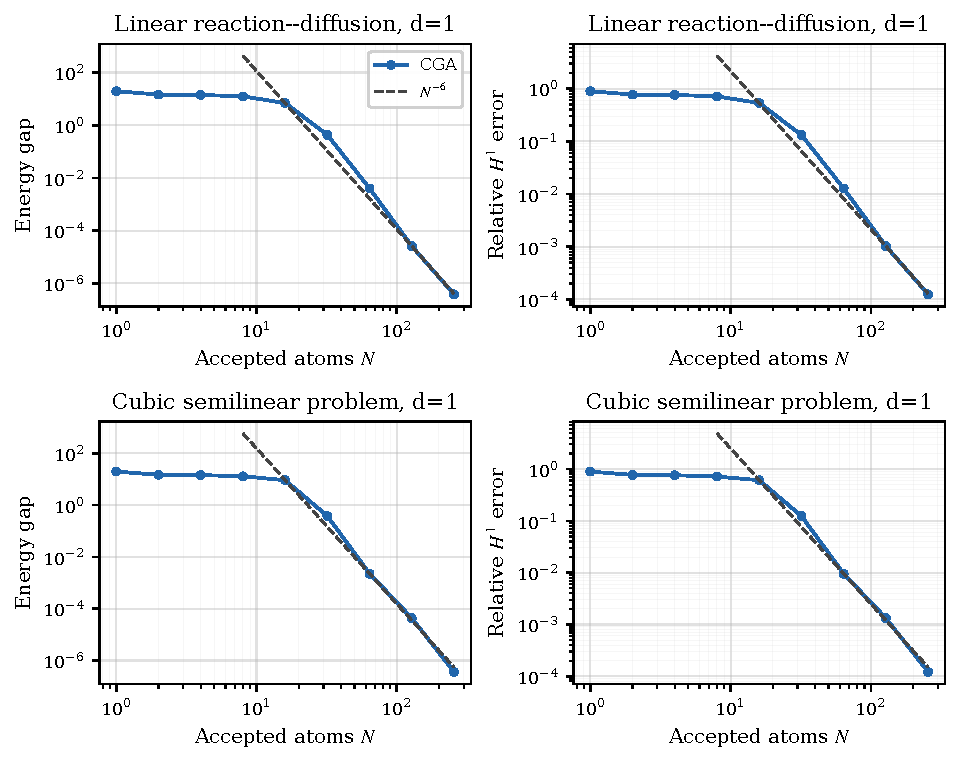
\includegraphics[width=0.96\textwidth]{cga_linear_cubic.pdf}
\caption{CGA values at accepted powers of two for the linear and cubic problems. Each dashed segment
is the corresponding metric-specific conditional guide of
\Cref{tab:window-orders}, restricted to the declared display window.}
\label{fig:cga-linear-cubic}
\end{figure}

\begin{table}[!htbp]
\centering\small
\caption{Dyadic errors for Linear reaction--diffusion, d=1.}
\label{tab:dyadic-01}
\begin{tabular}{@{}rrrrr@{}}
\toprule
$N$ & Energy gap & Order & Relative $H^1$ error & Order \\ \midrule
32 & $4.277\!\times\!10^{-1}$ & -- & $1.323\!\times\!10^{-1}$ & -- \\
64 & $3.983\!\times\!10^{-3}$ & $6.747$ & $1.277\!\times\!10^{-2}$ & $3.373$ \\
128 & $2.577\!\times\!10^{-5}$ & $7.272$ & $1.027\!\times\!10^{-3}$ & $3.636$ \\
256 & $3.801\!\times\!10^{-7}$ & $6.083$ & $1.247\!\times\!10^{-4}$ & $3.042$ \\
\bottomrule
\end{tabular}
\end{table}

\begin{table}[!htbp]
\centering\small
\caption{Dyadic errors for Cubic semilinear problem, d=1.}
\label{tab:dyadic-03}
\begin{tabular}{@{}rrrrr@{}}
\toprule
$N$ & Energy gap & Order & Relative $H^1$ error & Order \\ \midrule
32 & $3.752\!\times\!10^{-1}$ & -- & $1.239\!\times\!10^{-1}$ & -- \\
64 & $2.238\!\times\!10^{-3}$ & $7.389$ & $9.569\!\times\!10^{-3}$ & $3.694$ \\
128 & $4.301\!\times\!10^{-5}$ & $5.702$ & $1.326\!\times\!10^{-3}$ & $2.851$ \\
256 & $3.610\!\times\!10^{-7}$ & $6.896$ & $1.215\!\times\!10^{-4}$ & $3.448$ \\
\bottomrule
\end{tabular}
\end{table}



The two-dimensional sinh case is reported in the supplementary figures.  Its relative \(H^1\) error
decreases from \(4.074\times10^{-3}\) at \(N=256\) to \(1.990\times10^{-3}\) at \(N=512\), while the
local order decreases from 1.793 on \(128\to256\) to 1.034 on \(256\to512\). The final interval
therefore exhibits slower decay than the preceding interval.
\FloatBarrier

\subsection{Pure and regularized \texorpdfstring{\(p=4\)}{p=4} behavior}

\Cref{fig:cga-p4-representative} presents the one- and two-dimensional pure \(p=4\) cases using energy,
relative \(W^{1,4}\) error, and relative \(V\)-distance. The one-dimensional case reaches relative errors
\(1.579\times10^{-5}\) in \(W^{1,4}\) and \(1.680\times10^{-6}\) in the \(V\)-distance at its last
dyadic state \(N=128\). For the two-dimensional pure \(p=4\) problem, the interval \(128\to256\) has energy and \(V\)-orders 3.410 and
1.703.  On the final interval the \(V\)-distance continues to decrease, but the relative \(W^{1,4}\)
error increases from \(2.494\times10^{-3}\) to \(3.601\times10^{-3}\). Thus the terminal
Sobolev-error behavior is nonmonotone even though the \(V\)-distance decreases.

\begin{figure}[!htbp]
\centering
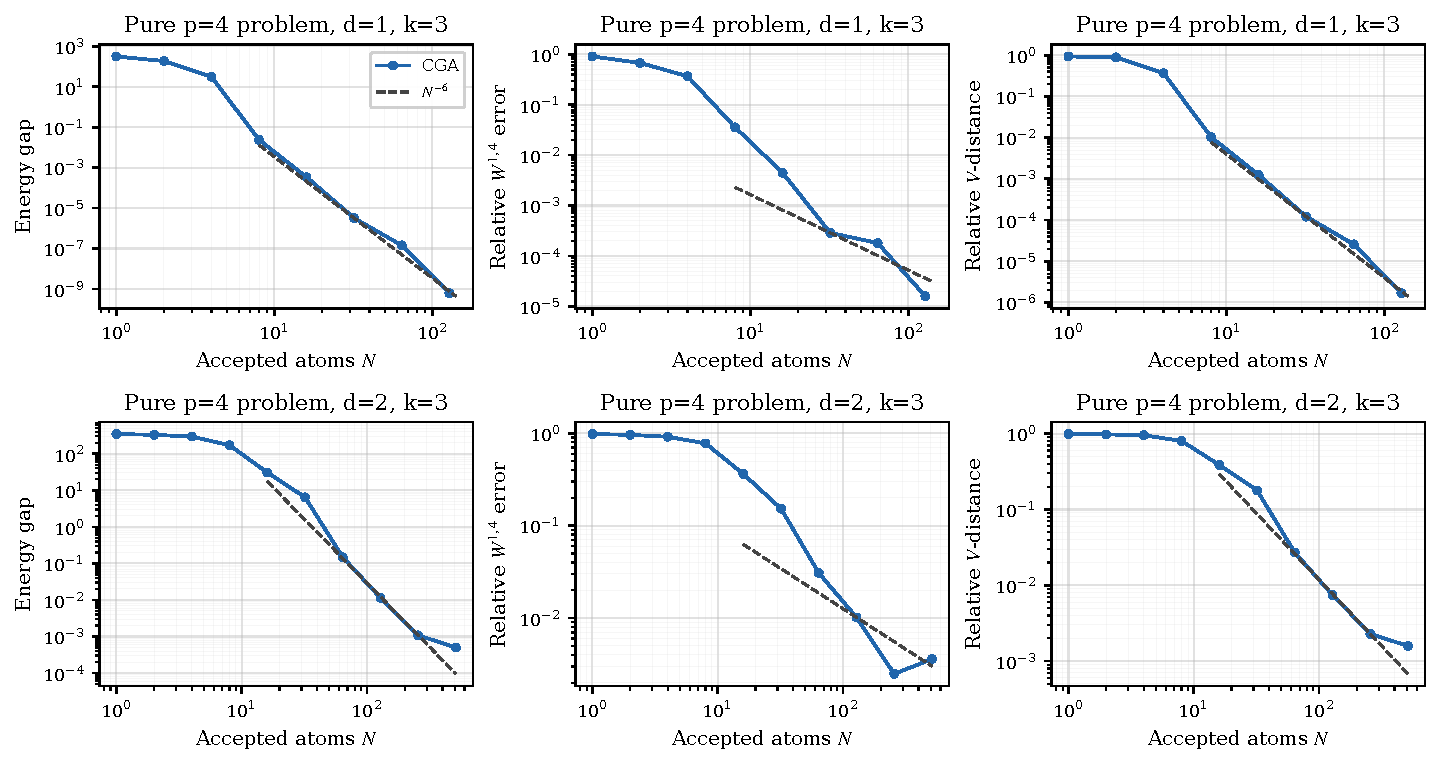
\includegraphics[width=0.98\textwidth]{cga_p4_representative.pdf}
\caption{CGA values at accepted powers of two for the representative one- and two-dimensional pure \(p=4\) problems. The
three columns show energy gap, relative \(W^{1,4}\) error, and relative \(V\)-distance. Dashed segments
use the metric-specific conditional exponents in \Cref{tab:window-orders}.}
\label{fig:cga-p4-representative}
\end{figure}

\begin{table}[!htbp]
\centering\scriptsize
\caption{Dyadic errors for Pure p=4 problem, d=1, k=3.}
\label{tab:dyadic-17}
\begin{tabular}{@{}rrrrrrr@{}}
\toprule
$N$ & Energy gap & Order & Relative $W^{1,4}$ & Order & Relative $V$ & Order \\ \midrule
8 & $2.363\!\times\!10^{-2}$ & -- & $3.567\!\times\!10^{-2}$ & -- & $1.028\!\times\!10^{-2}$ & -- \\
16 & $3.372\!\times\!10^{-4}$ & $6.131$ & $4.460\!\times\!10^{-3}$ & $2.999$ & $1.241\!\times\!10^{-3}$ & $3.051$ \\
32 & $3.180\!\times\!10^{-6}$ & $6.728$ & $2.869\!\times\!10^{-4}$ & $3.959$ & $1.205\!\times\!10^{-4}$ & $3.364$ \\
64 & $1.441\!\times\!10^{-7}$ & $4.464$ & $1.800\!\times\!10^{-4}$ & $0.672$ & $2.565\!\times\!10^{-5}$ & $2.232$ \\
128 & $6.187\!\times\!10^{-10}$ & $7.864$ & $1.579\!\times\!10^{-5}$ & $3.511$ & $1.680\!\times\!10^{-6}$ & $3.932$ \\
\bottomrule
\end{tabular}
\end{table}

\begin{table}[!htbp]
\centering\scriptsize
\caption{Dyadic errors for Pure p=4 problem, d=2, k=3.}
\label{tab:dyadic-08}
\begin{tabular}{@{}rrrrrrr@{}}
\toprule
$N$ & Energy gap & Order & Relative $W^{1,4}$ & Order & Relative $V$ & Order \\ \midrule
16 & $3.070\!\times\!10^{1}$ & -- & $3.624\!\times\!10^{-1}$ & -- & $3.862\!\times\!10^{-1}$ & -- \\
32 & $6.476\!\times\!10^{0}$ & $2.245$ & $1.528\!\times\!10^{-1}$ & $1.247$ & $1.786\!\times\!10^{-1}$ & $1.113$ \\
64 & $1.479\!\times\!10^{-1}$ & $5.452$ & $3.078\!\times\!10^{-2}$ & $2.311$ & $2.701\!\times\!10^{-2}$ & $2.725$ \\
128 & $1.140\!\times\!10^{-2}$ & $3.697$ & $1.017\!\times\!10^{-2}$ & $1.598$ & $7.452\!\times\!10^{-3}$ & $1.858$ \\
256 & $1.073\!\times\!10^{-3}$ & $3.410$ & $2.494\!\times\!10^{-3}$ & $2.028$ & $2.288\!\times\!10^{-3}$ & $1.703$ \\
512 & $4.975\!\times\!10^{-4}$ & $1.109$ & $3.601\!\times\!10^{-3}$ & $-0.530$ & $1.584\!\times\!10^{-3}$ & $0.531$ \\
\bottomrule
\end{tabular}
\end{table}



To examine the transition from uniformly elliptic regularizations to the pure model on one common
finite window, \Cref{fig:cga-epsilon-scan} compares \(\varepsilon=0,10^{-2},10^{-1},1\) for
\(p=4,d=1,k=3\).  At \(N=32\), the four relative \(W^{1,4}\) errors lie between
\(3.209\times10^{-4}\) and \(3.261\times10^{-4}\), while the relative \(V\)-distances lie between
\(9.518\times10^{-5}\) and \(1.198\times10^{-4}\).  The spread of these values indicates weak
dependence on the regularization over this parameter range and window, and it does not establish
coercivity of the unregularized Hessian on the full energy space.

\begin{figure}[!htbp]
\centering
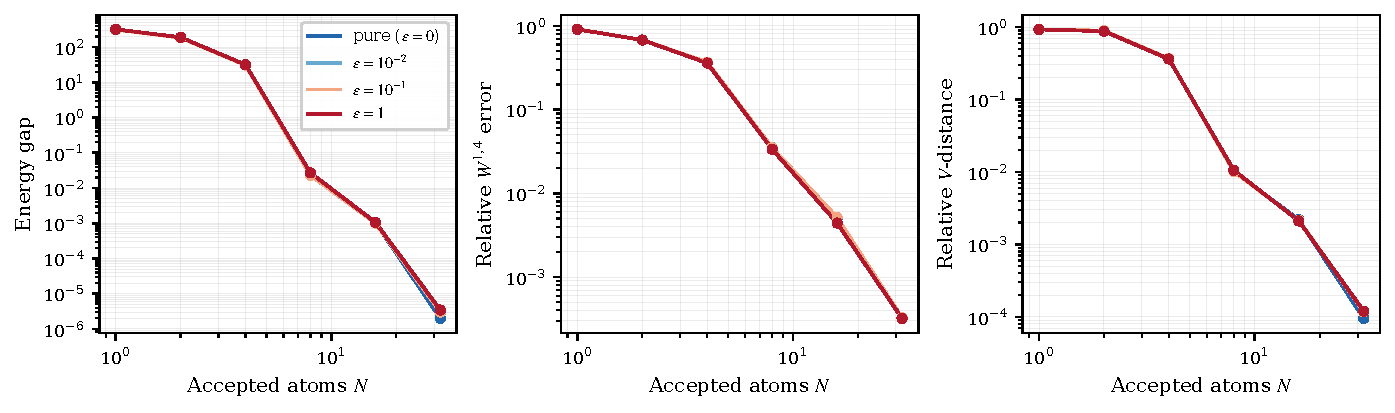
\includegraphics[width=0.98\textwidth]{cga_epsilon_scan.pdf}
\caption{Pure and regularized \(p=4,d=1,k=3\) CGA trajectories for four values of \(\varepsilon\).
Only dyadic accepted states are connected. All runs use the same target width and evaluator.}
\label{fig:cga-epsilon-scan}
\end{figure}

The regularized and reaction \(p=4\) trajectories are shown in
the supplementary figures.  As in the pure two-dimensional case, their final \(W^{1,4}\) errors
increase while their \(V\)-distances continue to decrease.  The same nonmonotone terminal behavior
therefore appears in all three \(p=4\) structures.
\FloatBarrier

\subsection{Finite-trajectory bounds and fractional innovation for the quartic models}
\label{sec:finite-trajectory-numerics}
\label{sec:fractional-innovation-p4}

We evaluate the estimates of \Cref{sec:c5} on the one-dimensional pure and
regularized \(p=4\), \(k=3\) trajectories, with \(u^*(x)=\cos(2\pi x)\) and
\(\varepsilon=0\) or \(0.1\) (cases \texttt{base\_pure} and \texttt{epsilon\_01}
in Supplement S1). These runs use a larger pool and a smaller accepted-state budget than the
eight cases of \Cref{sec:numerics}. The inner product held fixed during the estimates is
\[
 a_*(v,w)=\int_0^1\big(\varepsilon^2+3|(u^*)'|^2\big)v'w'\dd x.
\]
The calibration range contains the 25 retained states \(N=8,\ldots,32\) and its 24 transitions
\(N\to N+1\), \(N=8,\ldots,31\).  The subsequent finite range contains the 32 transitions
\(N\to N+1\), \(N=32,\ldots,63\), generated by extending the same previously computed iterates to \(N=64\).
The two transition sets are kept separate: all source, comparison, and fractional-innovation
constants are estimated on the calibration range only, while the continuation is used only as a
auxiliary numerical test.
At the starting index, the fixed auxiliary dictionary comprises 463 valid candidates and the first 128
valid reference atoms in the order in which they were generated, drawn with a separate seed. They
need not be linearly independent. Symmetry and the frozen normalization follow the theory, and
Supplement S2 specifies the ordering and the filtering. The reference atoms enter the estimates
only. Source coefficients are constructed from the starting-index residual and are not adjusted to fit
later errors.

The full active-space projections use untruncated QR on a common breakpoint-segmented Gauss
rule of order 20, cross-checked at order 16. The active linear systems have condition numbers
between \(7.7\times10^1\) and \(4.1\times10^3\). The maximum defect in
\cref{eq:c5-quartic} is below \(8.7\times10^{-17}\), and the projection-drop identity
has residual below \(1.5\times10^{-12}\). These are floating-point calculations, not interval
enclosures of the exact integrals or projections.

\paragraph{Source bound and Hessian-transfer conditions.}
\Cref{tab:merged-trajectory-conditions} collects the source data, the quartic comparison
constants, and the initial-value bounds of \Cref{thm:c5-source}, evaluated with
\(\underline\theta_m=\theta_m\), the observed selection ratio. In the table,
\(B=B_{\rm entry}\) and \(q=q_{\rm corr}\). The source energy
bounds at \(N=32\) are \(2.23\times10^{-2}\) and \(2.11\times10^{-2}\), compared with
energy gaps \(1.99\times10^{-6}\) and \(3.01\times10^{-6}\). Thus the source remainder
does not make this bound sharp; the accumulated-innovation contribution remains dominant.
For both models, \(\sigma^2/r_8^2\) is approximately \(6.21\times10^{-5}\), whereas
\(\sigma^2/r_{32}^2\) is \(0.751\) for the pure model and \(0.495\) for the regularized model.

\begin{table}[!htbp]
\centering
\small
\caption{Source and quartic comparison quantities on all retained states \(N=8\)--32. The source is fixed at the starting index; \(q\) and \(\rho\) are calibration-range maxima on \(N=8\)--32. Values are floating-point estimates.}
\label{tab:merged-trajectory-conditions}
\begin{tabularx}{\linewidth}{@{}Xrr@{}}
\toprule
Quantity & Pure \(p=4\) & \(\varepsilon=0.1\) \\
\midrule
Source budget \(B\) & \(4.361\times10^{1}\) & \(4.362\times10^{1}\) \\
Source remainder \(\sigma\) & \(1.726\times10^{-3}\) & \(1.728\times10^{-3}\) \\
\(\mathcal W_{24}\) & \(1.912\times10^{4}\) & \(2.913\times10^{4}\) \\
\(q=\max D_N/r_N\) & \(4.733\times10^{-2}\) & \(4.715\times10^{-2}\) \\
\(\rho=\max |R_N|/(r_N^2+D_N^2)\) & \(2.006\times10^{-2}\) & \(1.997\times10^{-2}\) \\
Computed \(r_{32}^2\) & \(3.969\times10^{-6}\) & \(6.025\times10^{-6}\) \\
Initial-value source bound for \(r_{32}^2\) & \(4.280\times10^{-2}\) & \(4.057\times10^{-2}\) \\
Computed energy gap at \(N=32\) & \(1.985\times10^{-6}\) & \(3.013\times10^{-6}\) \\
Initial-value source energy bound & \(2.231\times10^{-2}\) & \(2.114\times10^{-2}\) \\
\bottomrule
\end{tabularx}
\end{table}


For comparison with the finite-range discussion, the minimum active-space generalized Hessian
eigenvalues relative to the \(H^1\) Gram matrix are \(0.1328\) and \(0.1428\), and the
minimum finite-reference-pool selection ratios are \(0.9876\) and \(0.9911\).
Nevertheless, the sufficient lower bound of \cref{eq:c5-finite-margin} is negative at all 24
transitions in both models. Positive active-space spectra and finite-reference-set ratios therefore do
not establish the continuous relative-score condition. The selected directions remain valid for the
finite numerical experiment, but the transfer proposition cannot be invoked from these quantities alone.
The direct projection estimates below use the selected directions themselves and do not require that
sufficient lower bound to be positive.
The decomposition in \Cref{tab:transfer-margin-example} shows one representative transition.  The Hessian-transfer lower bound is negative even though the corresponding transition is retained; the score-quadrature and active-optimization terms are negligible at this step relative to the nonlinear-to-frozen defect.
\begin{table}[!htbp]
\centering
\scriptsize
\caption{One-step error-budget decomposition at the first calibration transition. The negative margin is a diagnostic: the nonlinear-to-frozen defect dominates the available frozen decrease even though the native step is accepted.}
\label{tab:transfer-margin-example}
\begin{tabularx}{\linewidth}{@{}Xrr@{}}
\toprule
Quantity & Pure \(p=4\), \(8\to9\) & Regularized \(\varepsilon=0.1\), \(8\to9\) \\
\midrule
Frozen decrease & \(1.8403\times10^{-2}\) & \(1.8175\times10^{-2}\) \\
Nonlinear-to-frozen defect & \(6.8347\times10^{-3}\) & \(6.8108\times10^{-3}\) \\
Score quadrature defect & \(9.73\times10^{-13}\) & \(9.95\times10^{-13}\) \\
Active optimization defect & \(4.36\times10^{-7}\) & \(4.48\times10^{-7}\) \\
Total score defect & \(6.8351\times10^{-3}\) & \(6.8112\times10^{-3}\) \\
Selection margin & \(-6.3599\times10^{-2}\) & \(-6.2742\times10^{-2}\) \\
\bottomrule
\end{tabularx}
\end{table}


\paragraph{Fractional-innovation calculation.}
For the benchmark \(\alpha=6\), fixed before evaluating the normalized drops, set
\begin{equation}
 x_N=r_N^2,\qquad
 \gamma_N=\sqrt{x_N-x_{N+1}},\qquad
 c_N=\frac{x_N-x_{N+1}}{x_N^{7/6}},\qquad N=8,\ldots,31.
 \label{eq:numerical-fractional-ratio}
\end{equation}
The minimum over all transitions is \(1.6904\times10^{-2}\) for the pure model and
\(1.0912\times10^{-2}\) for \(\varepsilon=0.1\); both occur at \(25\to26\).
Changing the quadrature order changes these stepwise ratios by less than
\(5.6\times10^{-12}\) relatively. Together with the computed \(q\) and \(\rho\), these
values permit a numerical evaluation of \cref{eq:c5-power,eq:c5-power-energy}.
Writing \(j=N-8\), the resulting finite-range comparison powers are
\[
 \widehat\delta_{8+j}=O(j^{-6}),\qquad
 d_{V,\bullet}(\widehat G_{8+j},u^*)=O(j^{-3}),\qquad
 \|\widehat G_{8+j}-u^*\|_{W^{1,4}}=O(j^{-3/2}),\quad 1\leq j\leq24.
\]
The explicit bound in \cref{eq:c5-power} also includes the starting state \(j=0\).
These powers describe a conditional envelope on the tested finite range, not a limit as \(N\to\infty\).

\begin{table}[!htbp]
\centering
\small
\caption{Fractional-innovation quantities for \(\alpha=6\), computed from every transition \(N\to N+1\), \(N=8,\ldots,31\). The fitted exponent describes the innovation score and is not used to choose the benchmark exponent or its bound.}
\label{tab:fractional-p4}
\begin{tabularx}{\linewidth}{@{}Xrr@{}}
\toprule
Quantity & Pure \(p=4\) & \(\varepsilon=0.1\) \\
\midrule
\(c_{\min}\) over all 24 transitions & \(1.690\times10^{-2}\) & \(1.091\times10^{-2}\) \\
Transition attaining \(c_{\min}\) & \(25\to26\) & \(25\to26\) \\
Fitted slope \(\nu\) of \(\log\gamma_N\) versus \(\log x_N\) & 0.5866 & 0.5898 \\
\(1/(2\nu-1)\) from the fit & 5.77 & 5.57 \\
Fractional bound for \(r_{32}^2\), \(\alpha=6\) & \(3.774\times10^{-2}\) & \(4.110\times10^{-2}\) \\
Fractional bound / computed \(r_{32}^2\) & \(9.510\times10^{3}\) & \(6.821\times10^{3}\) \\
Fractional energy bound at \(N=32\) & \(1.967\times10^{-2}\) & \(2.142\times10^{-2}\) \\
\bottomrule
\end{tabularx}
\end{table}


A least-squares fit of \(\log\gamma_N\) against \(\log x_N\), using all 24 transitions,
gives slopes \(\nu=0.5866\) and \(0.5898\). The relation
\(\alpha=1/(2\nu-1)\) associates these fitted innovation powers with \(5.77\) and
\(5.57\), respectively. This fit concerns \(\gamma_N=\theta_NS_N/\ell_N\), not \(S_N\)
alone; it does not independently establish either factor in \cref{eq:c5-power-factors}.

The worst-step constants still yield conservative terminal projection bounds:
\(3.77\times10^{-2}\) and \(4.11\times10^{-2}\), approximately
\(9.5\times10^3\) and \(6.8\times10^3\) times the computed projection errors.
The fractional bound is slightly smaller than the source bound for the pure model and slightly
larger for the regularized model. Positive drops on a finite sequence also give a positive
minimum normalized ratio for any fixed exponent. The computation establishes the stated numerical
envelope and its constants, but does not uniquely identify sixth-order decay or verify an
asymptotic mechanism. Such a conclusion would require bounds uniform over increasing index ranges.

\paragraph{Continuation beyond the calibration range.}
To test whether the calibrated constants remain informative immediately beyond the range on which
they were fixed, we continued the two trajectories from \(N=32\) to \(N=64\), keeping the same
candidate pools, previously computed iterates, and source coefficients and drawing no further random atoms. The
comparison exponent and all constants were kept at their \(N=8\)--\(32\) values. Most transitions in
this subsequent finite range satisfy the normalized-innovation sufficient condition with those constants.
At quadrature order \(20\), it holds for 27 of the 32 continuation transitions in the pure model
\(27/32=84.4\%\) and 28 of 32 in the regularized model
\(28/32=87.5\%\); only five and four transitions, respectively, fall
below the prescribed threshold. These exceptions concern the sufficient condition, not the validity
of the theoretical implication. In both models, the first such transition is \(N=33\to34\), and the
minimum ratio \(c_N/c_0\) over the continuation is \(0.156\) and \(0.187\), respectively; the
terminal squared projection errors are \(4.770\times10^{-7}\) and \(4.626\times10^{-7}\). The
order-16 cross-check changes these reported values only in the displayed last digits. The
continuation therefore shows that the calibrated condition remains satisfied for
most transitions, together with a substantial error decrease and agreement with the algebraic
identities on the subsequent states. The few exceptions prevent applying the same fixed-constant
theorem over the entire continuation range. The stated finite-range envelope therefore retains
its calibration range $N=8$--32, while the continuation provides supporting stepwise numerical
evidence without establishing an asymptotic rate.

\begin{table}[!htbp]
\centering\small
\caption{Continuation from $N=32$ to $N=64$ (32 transitions) with constants fixed on $N=8$--$32$. Pass counts refer to the normalized-innovation sufficient condition; the first failed transition starts at the reported $N$.}
\label{tab:continuation-window}
\begin{tabular}{@{}lrrrrr@{}}
\toprule
Model & New steps & Pass & First failed $N$ & $\min c_N/c_0$ & $r_{64}^2$ \\
\midrule
Pure $p=4$ & 32 & 27 & 33 & 0.156 & $4.770\times10^{-7}$ \\
$\varepsilon=0.1$ & 32 & 28 & 33 & 0.187 & $4.626\times10^{-7}$ \\
\bottomrule
\end{tabular}
\end{table}

\FloatBarrier


\section{Equal-DOF baseline comparisons}
\label{sec:results}

\subsection{Comparison setup and scope}

Five cases use a common evaluator: the one-dimensional linear problem, the one-dimensional cubic
problem, the two-dimensional sinh problem, the one-dimensional pure \(p=4\) problem, and the
two-dimensional pure \(p=4\) problem. The comparison variable is the number of independent global
coefficients: retained atoms for CGA, ridge features held fixed for RFM, and independent
finite-element coefficients after the constant mode is removed where required. Equal degrees of
freedom (DOF) do not imply equal runtime, memory, score evaluations, or nonlinear solver work, and
no cross-method timing conclusion is drawn from runs performed in different environments.
The supplementary numerical data at
\url{https://github.com/RonzolYu/cga4PDE} give the prescribed realization count, the
available converged realizations, and the solver status for each width.

FEM uses continuous Lagrange elements on uniform one-dimensional meshes or structured triangular
two-dimensional meshes.  P1 and P3 provide low- and high-order mesh-based references in the main
figures. P2 results are retained in the supplementary material. P3 is the most accurate among the tested uniform-mesh FEM variants
at each largest common coefficient count reported below. The linear and cubic FEM curves are close
at high resolution, which is consistent with the common manufactured profile and an \(H^1\) error
dominated by the finite-element approximation.

For each case, the RFM uses a nested family of normalized \(\relu^3\) ridges and fits the outer
coefficients. Ten random-feature realizations are prescribed for each problem. Curves show the median and
interquartile range over available converged realizations at each width, and the supplementary numerical data give
the prescribed count together with solver status. All ten
realizations reach the displayed ranges for the linear, cubic, sinh, and one-dimensional pure
\(p=4\) problems. In the two-dimensional pure \(p=4\) problem, seven realizations are available at
\(N=128\) and four are available at \(N=256\); consequently its statistical curve ends at 256 and its terminal band is based
on four available realizations.  No distributional statement is made at \(N=512\).

The CGA and RFM comparison curves join the computed powers of two listed in the numerical setup and the
terminal retained state needed to define the largest common comparison width, while FEM uses its own mesh degrees of
freedom. The figures contain no common-grid interpolants, theoretical reference lines, or
convergence-order-versus-DOF curves. The reported panel range ends at the terminal CGA width fixed
by the stopping rule, so that endpoint is determined by the stopping rule and the available method
states rather than by the plotted error values. Each method is shown only over the states it
actually reached. The equal-DOF tables use linear interpolation of log(error) against log(DOF)
between adjacent computed values when an exact coefficient count is unavailable; no extrapolation
is used.

\begin{table}[!htbp]
\centering
\small
\caption{Training and evaluation parameters for the equal-DOF comparison.}
\label{tab:protocol}
\begin{tabularx}{\textwidth}{@{}p{0.26\textwidth}X@{}}
\toprule
Component & Setting \\
\midrule
RFM & Nested \(\relu^3\) prefixes; the discrete homogeneous normalization defined in \Cref{sec:numerics}; centered for pure \(p\); ten prespecified random seeds, with prescribed and available-realization counts reported. \\
FEM & Continuous P1/P2/P3; structured meshes; assembly order 10, increased to 80 for the one-dimensional multifrequency cases; relative/absolute Newton tolerances \(10^{-11}\)/\(10^{-12}\). \\
Training quadrature & One dimension: 256 cells, order 6; two dimensions: \(63\times63\) cells, tensor-product order 3. \\
Evaluation quadrature & One dimension: 2048 cells, order 8; two dimensions: \(64\times64\) cell partition, order 3. \\
Independent refinement & One dimension: 3072 cells, order 8; two dimensions: \(80\times80\) cell partition, order 3. \\
Common DOFs & \(8,16,32,64,128,256\), with 512 used only when every method required by the comparison is bracketed by computed states. \\
\bottomrule
\end{tabularx}
\end{table}
\FloatBarrier

\subsection{Unified evaluator, retained states, and fixed denominators}

The comparison states are re-evaluated after training by a frozen evaluator that is separate from
the quadrature used to construct the features or fit their coefficients.  The main evaluation rule
uses the quadrature listed in \Cref{tab:protocol}; an independent refinement is used for the independently evaluated quantities.  Thus, a solver-specific status is not interpreted as an independent accuracy bound, and a state is not removed merely because an independently evaluated quantity is unavailable.  The
set of retained states and the denominator conventions are summarized in
\Cref{tab:unified-audit-boundary,tab:rfm-fixed-denominators}.

The common evaluation retains 617 stored states, comprising 612 newly generated states and five archived
terminal states.  All 617 satisfy their solver-specific acceptance criterion and the independent coefficient-count
check.  The stricter signed energy/metric evaluation admits 611 states, while the common \(H^1\)-dual
residual threshold admits 394; these are different filters and are reported with their own
denominators.  The independent two-dimensional Bregman calculation is an energy-integration evaluation
on 138 states, not a replacement for the residual or optimizer checks.

For random-feature comparisons, the prescribed denominator is ten seeds at every configured width.
The displayed median and interquartile range are computed only from evaluated states that pass the
metric-specific checks, whereas missing rank-budget states remain failures in the \(10\)-seed
denominator.  In particular, the three C3 states missing at \(N=256\), the one C5 state missing at
\(N=128\), and the two C5 states missing at \(N=256\) are not dropped before forming success counts.
All other displayed RFM widths have \(10/10\) evaluated states; their strict residual counts can
still be smaller because residual qualification is a separate filter.

\begin{table}[!htbp]
\centering
\small
\caption{Unified re-evaluation boundaries and fixed denominators for the archived comparison states.}
\label{tab:unified-audit-boundary}
\begin{tabularx}{\textwidth}{@{}p{0.42\textwidth}X@{}}
\toprule
Audit item & Count or convention \\
\midrule
Retained states in the common audit & 617 total: 612 newly generated; 5 archived terminal \\
Native solver acceptance & (617/617); this records the native acceptance rule only \\
Independent coefficient-count check & (617/617) \\
Signed energy/metric audit & (611/617); six states remain excluded from the corresponding strict energy summary \\
Common H1-dual residual, threshold 2e-6 & (394/617); this is reported separately from native acceptance \\
Independent two-dimensional Bregman-energy audit & (137/138); this tests energy-integration stability and is not an optimization certificate \\
\bottomrule
\end{tabularx}
\end{table}

\begin{table}[!htbp]
\centering
\scriptsize
\caption{Prescribed random-feature denominators at widths where states are missing or further audit filtering is active.  A missing state remains in the denominator.}
\label{tab:rfm-fixed-denominators}
\begin{tabularx}{0.98\textwidth}{@{}lrrrr>{\raggedright\arraybackslash}X@{}}
\toprule
Case/width & Plan & Eval. & Missing & Energy & Strict H1 residual \\
\midrule
C3, (N=256) & 10 & 7 & 3 & (7/10) & (0/10) \\
C5, (N=128) & 10 & 9 & 1 & (9/10) & (0/10) \\
C5, (N=256) & 10 & 8 & 2 & (7/10) & (0/10) \\
\bottomrule
\end{tabularx}
\end{table}

\FloatBarrier

\subsection{Relative Sobolev errors}

For the linear, cubic, and sinh problems,
\Cref{fig:baseline-sobolev-1d,fig:baseline-sobolev-rest} report the relative \(H^1\) error. For the
two pure \(p=4\) problems, the corresponding panels report the relative
\(W^{1,4}\) error. These are Sobolev errors; the natural \(V\)-distance is reported separately below.

\begin{figure}[!htbp]
\centering
\begin{subfigure}[t]{0.49\textwidth}
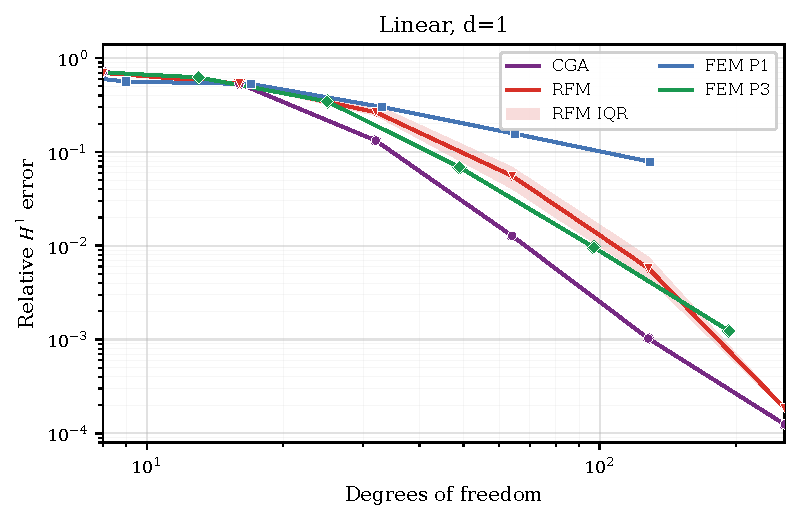
\includegraphics[width=\linewidth]{C1_relative_h1_error.pdf}
\caption{Linear, \(d=1\).}
\end{subfigure}\hfill
\begin{subfigure}[t]{0.49\textwidth}
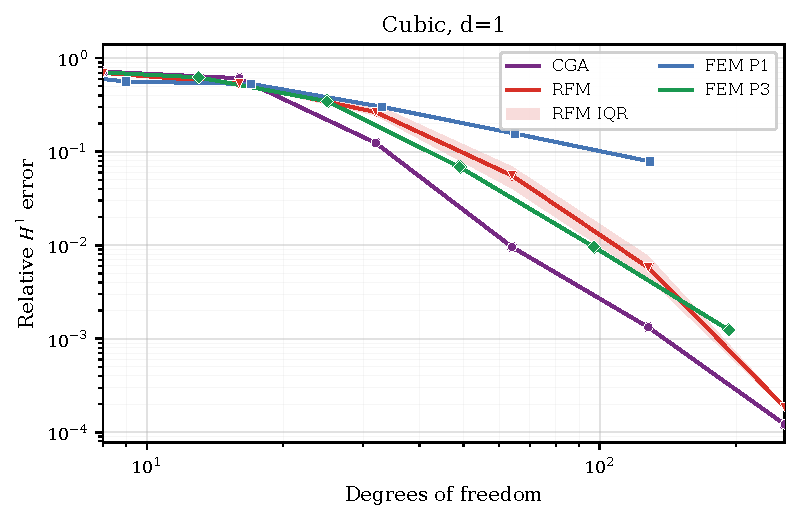
\includegraphics[width=\linewidth]{C2_relative_h1_error.pdf}
\caption{Cubic, \(d=1\).}
\end{subfigure}
\caption{Relative \(H^1\) error versus effective degrees of freedom for the one-dimensional
multifrequency problems. RFM curves show medians and interquartile bands over successful realizations
from ten prespecified runs. All markers are computed states.}
\label{fig:baseline-sobolev-1d}
\end{figure}

\begin{figure}[!htbp]
\centering
\begin{subfigure}[t]{0.32\textwidth}
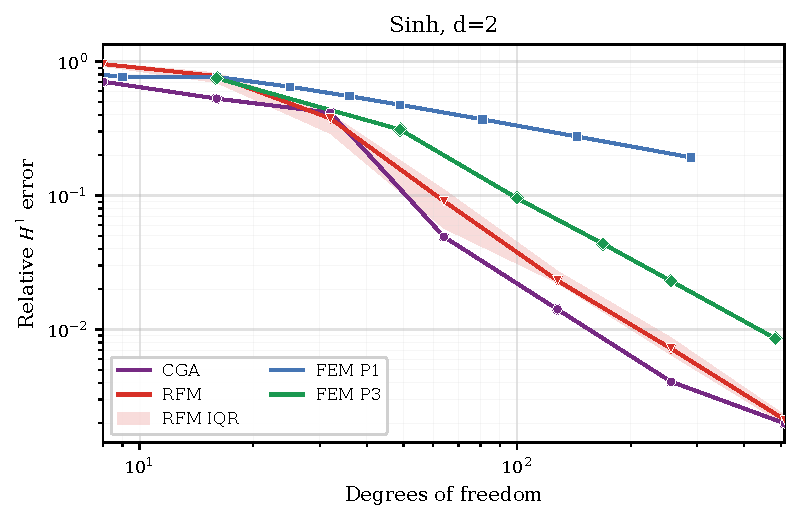
\includegraphics[width=\linewidth]{C3_relative_h1_error.pdf}
\caption{Sinh, \(d=2\): relative \(H^1\) error.}
\end{subfigure}\hfill
\begin{subfigure}[t]{0.32\textwidth}
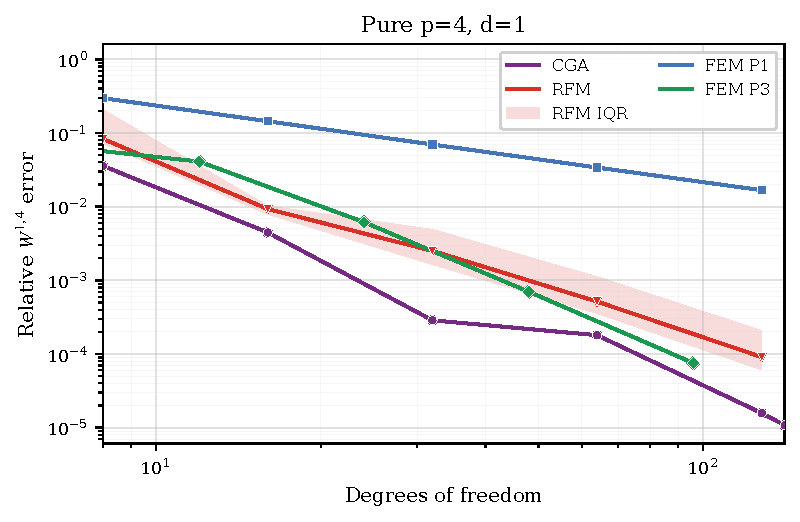
\includegraphics[width=\linewidth]{C4_relative_w1p_error.pdf}
\caption{Pure \(p=4\), \(d=1\): relative \(W^{1,4}\) error.}
\end{subfigure}\hfill
\begin{subfigure}[t]{0.32\textwidth}
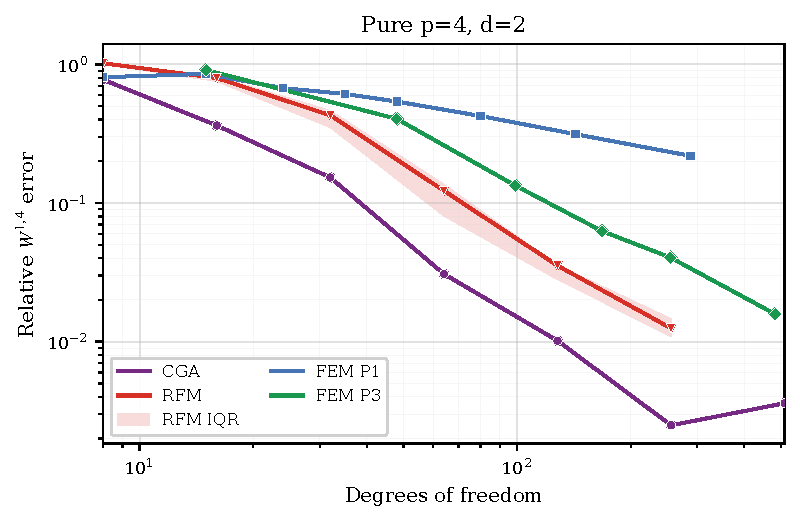
\includegraphics[width=\linewidth]{C5_relative_w1p_error.pdf}
\caption{Pure \(p=4\), \(d=2\): relative \(W^{1,4}\) error.}
\end{subfigure}
\caption{Relative Sobolev errors for the two-dimensional sinh problem and the pure \(p=4\) problems.
The two-dimensional pure \(p=4\) RFM band is formed from the available realizations; its statistics at \(N=128\) and 256 use
seven and four available realizations, respectively.}
\label{fig:baseline-sobolev-rest}
\end{figure}
\FloatBarrier

At the largest common endpoint supported by the configured RFM widths and bracketing FEM states,
CGA has the smallest relative Sobolev error in the linear, cubic, sinh, and one-dimensional pure
\(p=4\) problems, for which all ten prescribed RFM solves succeeded.
The RFM-median/CGA ratios are 1.49, 1.52, 1.77, and 5.76, and the P3/CGA ratios are 4.24, 4.35, 5.64,
and 1.88. In the two-dimensional pure \(p=4\) problem the successful-run RFM median and the P3 value
are also above the CGA value, by factors
5.01 and 16.12, respectively, but the RFM statistic is based on only four of ten prescribed solves.
These are endpoint comparisons at equal coefficient count. The curves cross at smaller widths in
some cases, so the data do not support uniform dominance at every DOF.

\begin{table}[!htbp]
\centering\scriptsize
\caption{Relative Sobolev error at the largest common coefficient count reported for each problem. RFM statistics use successful realizations from ten prescribed runs and are reported as median [Q1,Q3]. The first four problems have ten successful runs; the two-dimensional pure \(p=4\) row is conditional on four successful runs and is not included in an aggregate ranking. Ratios larger than one favor CGA.}
\label{tab:baseline-terminal}
\begin{tabular}{@{}crrrrrr@{}}
\toprule
Problem & DOF & CGA & RFM median [Q1,Q3] & Success & RFM/CGA & FEM P3/CGA \\ \midrule
Linear, d=1 & 256 & $1.247\!\times\!10^{-4}$ & $1.853\!\times\!10^{-4}$ [$1.779\!\times\!10^{-4}$, $1.913\!\times\!10^{-4}$] & 10/10 & 1.49 & 4.24 \\
Cubic, d=1 & 256 & $1.215\!\times\!10^{-4}$ & $1.853\!\times\!10^{-4}$ [$1.779\!\times\!10^{-4}$, $1.913\!\times\!10^{-4}$] & 10/10 & 1.52 & 4.35 \\
Sinh, d=2 & 256 & $4.074\!\times\!10^{-3}$ & $7.195\!\times\!10^{-3}$ [$6.472\!\times\!10^{-3}$, $8.663\!\times\!10^{-3}$] & 10/10 & 1.77 & 5.64 \\
Pure p=4, d=1 & 128 & $1.579\!\times\!10^{-5}$ & $9.103\!\times\!10^{-5}$ [$6.108\!\times\!10^{-5}$, $2.077\!\times\!10^{-4}$] & 10/10 & 5.76 & 1.88 \\
Pure p=4, d=2 & 256 & $2.494\!\times\!10^{-3}$ & $1.248\!\times\!10^{-2}$ [$1.087\!\times\!10^{-2}$, $1.465\!\times\!10^{-2}$] & 4/10 & 5.01 & 16.12 \\
\bottomrule
\end{tabular}
\end{table}

\FloatBarrier

\subsection{Natural \texorpdfstring{\(V\)}{V}-distance for the \texorpdfstring{\(p\)}{p}-models}

\Cref{fig:baseline-v} repeats the two pure \(p=4\) comparisons with the relative \(V\)-distance defined in
\Cref{sec:numerics}.  Keeping this geometry separate from the \(W^{1,4}\) error is important because the
two quantities need not have the same terminal behavior.  The figure uses the same computed-state and
RFM uncertainty conventions as the Sobolev panels.

\begin{figure}[!htbp]
\centering
\begin{subfigure}[t]{0.49\textwidth}
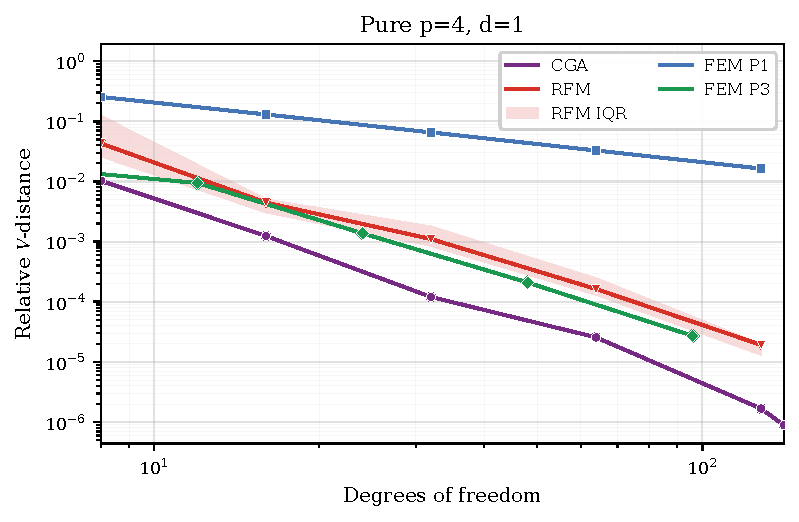
\includegraphics[width=\linewidth]{C4_v_distance.pdf}
\caption{Pure \(p=4,d=1\).}
\end{subfigure}\hfill
\begin{subfigure}[t]{0.49\textwidth}
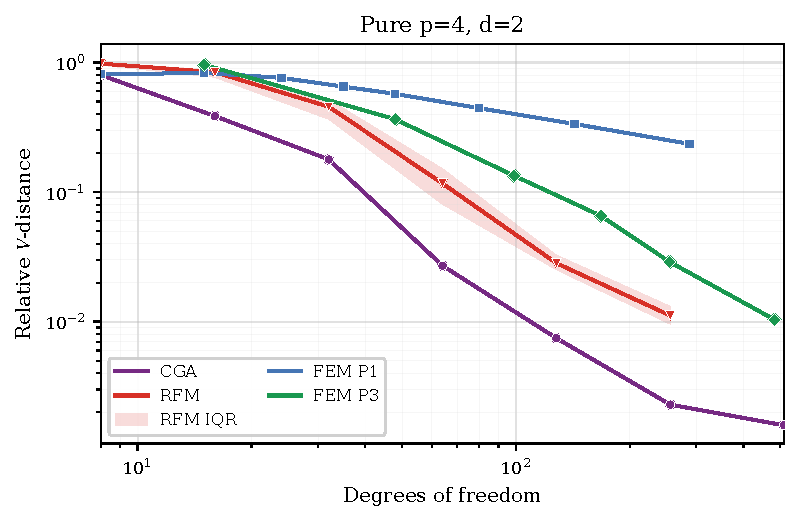
\includegraphics[width=\linewidth]{C5_v_distance.pdf}
\caption{Pure \(p=4,d=2\).}
\end{subfigure}
\caption{Relative \(V\)-distance versus effective degrees of freedom.  No theoretical reference line
or common-grid interpolation is drawn.}
\label{fig:baseline-v}
\end{figure}
\FloatBarrier

\subsection{Interpretation limits}

The equal-DOF results compare finite-pool CGA with the specified FEM and RFM implementations.  They do
not establish a runtime ordering, do not compare CGA with every randomized or greedy dictionary method,
and do not turn endpoint ratios into asymptotic complexity estimates. The two-dimensional pure
\(p=4\) RFM summaries use
the four available realizations at the terminal width and are not used as a complete ten-run statistical
comparison. Supplementary energy-gap comparisons are more sensitive to quadrature because they
subtract two separately integrated energies. The supplementary numerical data specify the prescribed and
converged realization counts, interpolation brackets, and computed coefficient counts.

\section{Discussion and conclusion}
\label{sec:discussion}

The atomic source condition and directional smoothness yield an \(O(m^{-1})\) energy bound
for the ideal continuous-dictionary CGA. For finite-pool CGA, continuous-dictionary coverage
enters multiplicatively, whereas score evaluation, radial stationarity, and coefficient
optimization introduce distinct additive errors. The one-step inequality specifies the relative
accuracy conditions under which the same energy order is retained.

For standard pure, regularized, and reaction \(p\)-energies with \(p\geq2\), the energy gap
is equivalent to the squared natural distance and controls the \(p\)-th power of the Sobolev
error. An energy exponent \(\alpha\) therefore gives natural-distance and Sobolev exponents
\(\alpha/2\) and \(\alpha/p\). This conclusion uses the pointwise structure of the energy
density; a general convex density with \(p\)-growth need not satisfy the same equivalence.

The sharper estimates in \Cref{sec:c5} require additional assumptions. Residual
comparison relates the dictionary seminorm to the full dual norm. Local Hessian transfer
requires coercivity, a dictionary norm bridge, relative score resolution, and source and entropy
bounds after restart. The finite-trajectory estimates use the projections onto the computed
spaces, together with either an approximate source representation or a
fractional lower bound on the normalized innovations. The quartic energy decomposition relates
both projection estimates to nonlinear energy errors.

The concrete semilinear family in \Cref{sec:c5-hessian} makes the nonlinear interface explicit.  Its
$C_{\rm emb}$, $L_\lambda$, $C_\lambda$, and $B_\lambda$ constants give a computable candidate
margin $\Delta_\lambda$ with the required $C_\lambda^2$ factor.  The Route-A closure certificate
then requires the same projected, unrenormalized restarted dictionary to satisfy a quantitative entropy
bound and requires every declared state to remain in the Hessian ball.  These checks are now isolated
as falsifiable obligations; the manuscript does not call them an unconditional theorem before they
are verified.

The one-dimensional pure and regularized quartic calculations evaluate these quantities at
every accepted state on \(N=8\)--32 and continue the same prefixes through \(N=64\) with the
constants held fixed. Active-space Hessian spectra are positive, but the
sufficient selection margins are negative throughout this window. The continuous
Hessian-transfer hypotheses are therefore unverified. The direct projection and energy
identities agree to floating-point accuracy under two quadrature rules. Both the source and
fractional-innovation bounds cover the computed errors, although the terminal bounds remain
several thousand times larger. With the prescribed exponent \(\alpha=6\), the latter yield
finite-window comparison powers \(6\), \(3\), and \(3/2\) for energy, natural distance, and
\(W^{1,4}\) error. The fitted innovation powers are descriptive: positivity on a finite
trajectory neither determines a unique decay exponent nor gives constants uniform over
increasing widths. In the continuation, the normalized-innovation sufficient condition holds
on most transitions: 27 of 32 for the pure model and 28 of 32 for the regularized model.
The few exceptions preclude a uniform application of the frozen-constant bound across the
extended window, so the continuation remains a stepwise diagnostic.

At the largest common coefficient count, CGA has the smallest relative Sobolev error in the
four comparisons after filtering to the reported converged RFM realizations. The same ordering holds in the
two-dimensional pure \(p=4\) example, where only four of ten prescribed RFM realizations reach the terminal
width. These comparisons concern the specified implementations and coefficient counts;
they establish neither an ordering at every width nor a runtime advantage.

The remaining work is therefore specific: close the three Route-A gates for a declared nonzero $\lambda$ range,
or switch to the error-decomposition controller described in the revision plan.  More examples alone
would not close these gates.  Reliable numerical enclosures and comparisons with a common
computational-work measure would provide additional evidence beyond the finite-window comparisons
reported here.


\appendix
\section{Proof of the one-dimensional source estimate}
\label{app:source}

We give the details of \Cref{prop:1dsource} because it provides a concrete source class without
appealing to a multivariate variation-space theorem. The Sobolev representative of
\(v\in W^{k+1,1}(0,1)\) satisfies the integral remainder identity
\begin{equation}
 v(x)=\sum_{j=0}^k\frac{v^{(j)}(0)}{j!}x^j
 +\frac1{k!}\int_0^1 v^{(k+1)}(t)(x-t)_+^k\dd t.
 \label{eq:integral-remainder}
\end{equation}
By hypothesis, the polynomial part is a finite linear combination of fully active ridges. The
coefficients are bounded by a constant times \(\sum_{j=0}^k\abs{v^{(j)}(0)}\), where the constant
accounts for the conditioning of the fixed basis of \(\mathbb P_k\), the space of polynomials of
degree at most \(k\). It also depends on the chosen Sobolev norm and on the fixed exponent \(p\);
rescaling the interval would change it.

For the second term, the map
\[
 [0,1]\ni t\longmapsto (\cdot-t)_+^k\in W^{1,p}(0,1)
\]
is continuous for \(k\geq1\). Indeed, both the function and its first weak derivative depend
continuously on the translation parameter in the corresponding \(L^p\) spaces. Hence the integral in
\cref{eq:integral-remainder} is a Bochner integral. Approximate
\(v^{(k+1)}(t)\dd t/k!\) by signed simple measures. The associated finite sums of truncated powers
converge in \(W^{1,p}\), and their total coefficient variation is bounded by
\(\norm{v^{(k+1)}}_{L^1}/k!\). Passing to the atomic closure and including the upper normalization factor
proves \Cref{prop:1dsource}.

The argument also shows why \(k\geq1\) is used when the ambient space is \(W^{1,p}\): a discontinuous
step activation does not have the required translation continuity in that norm. It shows in addition
why the multivariate case is not obtained by replacing \(t\) with a hyperplane parameter, since the
representation and the variation measure then have a different geometry.


\footnotesize
\bibliographystyle{plainnat}
\ifdefined\CGAFromRoot
\bibliography{tex/References/references}
\else
\bibliography{References/references}
\fi

\end{document}
